% documentclass options:
% a4paper | letterpaper | ...  - paper size
% 10pt | 11pt | 12pt           - font size
% onecolumn | twocolumn        - toggle two columns
% titlepage | notitlepage      - toggle title page
% oneside | twoside            - toggle styling for two-side printing
% landscape                    - create landscape document instead
% draft                        - indicate formatting issues
% fleqn                        - left-align formulas
% leqno                        - put formula numbering on the left hand side instead of right
\documentclass[12pt, a4paper, notitlepage, oneside]{article}
\usepackage[margin=2cm]{geometry} % set page margins
\usepackage[utf8]{inputenc}

% line spacing. confusingly, use 1.3 for one-and-a-half, and 1.6 for double spacing
\linespread{1.0}

% replace paragraph indent with vertical spacing
\usepackage{parskip}
%\setlength{\parindent}{15pt} % reinstate paragraph indent

% Use \reindent at the start of a paragraph to indent it instead
\newcommand{\reindent}[1]{{\setlength{\parindent}{15pt}\setlength{\parskip}{0pt}#1}}

\usepackage{xcolor} % colors
\usepackage{graphicx}
\usepackage{hyperref} % URLs

%%% math tools and symbols %%%
\usepackage{xfrac}
\usepackage{amsfonts}
\usepackage{amssymb}
\usepackage{stmaryrd}
\usepackage{mathtools}
%\mathtoolsset{showonlyrefs} % only label equations that are referenced

\usepackage{listings}
\lstdefinestyle{typewriter}{
    showspaces=false,
    showstringspaces=false,
    basicstyle=\normalsize\ttfamily,
    breaklines=true,
    keepspaces=true
}
\lstset{style=typewriter}

%%%%% Project-specific settings %%%%%
\usepackage{tikz}
\usetikzlibrary{arrows.meta}
\usetikzlibrary{positioning}
%%%%% End project-specific settings %%%%%

% change paragraph
\begin{document}
    % control the depth for showing section numbering and including in the table of contents
    %  5: subparagraph
    %  4: paragraph
    %  3: subsubsection
    %  2: subsection
    %  1: section
    %  0: chapter
    % -1: part
    % for example, set secnumdepth 0 to remove numbers from an entire article
    \setcounter{secnumdepth}{3}
    \setcounter{tocdepth}{3}

    % change document-wide paragraph alignment
    %\raggedright % Left justified
    %\raggedleft  % Right justified
    %\centering   % Center

    %\frenchspacing % remove extra spacing after periods
    \nonfrenchspacing

    \title{Reversible Integer FFT \\ \textit{PAT Project 2022}}
    \author{Troels Korreman Nielsen (xck773)}
    \date{\today}
    \maketitle
    %\begin{abstract}
    %    The Fast Fourier Transform (FFT) is a widely-used algorithm for approximating the
Fourier Transform of a function.
FFT and its derivatives have a variety of practical uses in
mathematics, physics, signal processing, and many related fields.
For example,
the related Discrete Cosine Transform is employed in common media compression formats such as
MP3, JPEG, and MP4.

Especially in the cases of compression and de-noising,
we are interested in utilizing both the forward and inverse versions of the transform.
FT is an injective function with a well-defined inverse transformation (IFT),
but designing an approximation that retains this property presents some challenges.
%
In this report,
a reversible Fast Fourier Transform algorithm is presented
that can be directly implemented in a reversible language.
The ability to implement the algorithm in such a language can serve as proof of injectiveness.
Furthermore, deriving the inverse transform from the forward transform can ensure
that there are zero discrepancies between the two.

    %\end{abstract}
    \tableofcontents
    %\listoffigures
    %\listoftables
    \newpage

    %%%%% \input or \include statements go here %%%%%
    \section{The Fourier Transform}

\begin{equation}
     \hat g(k) = \int_{-\infty}^{\infty} g(x) \cdot e^{-2 \pi i k x} dx
\end{equation}

\begin{equation}
     \hat g(k) = \int_{x_1}^{x_2} g(x) \cdot e^{-2 \pi i k x} dx \cdot (t_2 - t_1)
\end{equation}

\subsection{Discrete Fourier Transform}

\begin{equation}
    X(k) = \sum_{n = 0}^{N - 1} x(k) \cdot e^{-2 \pi i kn / N}
\end{equation}

    \section{Fast Fourier Transform}

The time cost complexity of naively computing the DFT of a signal is $O(N^2)$.
Luckily, by exploiting certain inherent properties of the transform,
we can reduce this to $O(N \log N)$ while greatly reducing the needed number of multiplications.

\subsection{Twiddle factor}

To simplify the representation and computation of the DFT,
we define the following constant:

\begin{equation}
    W_N = e^{-2 \pi i / N}
\end{equation}

This is often referred to as the \textit{twiddle factor}.
When the parameter $N$ isn't specified,
it should be inferred contextually.

Using this, we can then rephrase the DFT as:
\begin{equation}
    X(k) = \sum_{n = 0}^{N - 1} W_N^{nk} x(n)~~,~~k \in [0; N)
\end{equation}

\subsection{Periodicity and symmetry}

Some properties of the twiddle factor are exploited in order to minimize the amount of operations
and develop an $O(n \log n)$ algorithm for computing the DFT.
In order to understand these,
we must take a closer look at the twiddle factor and what it actually means.

We can express this succinctly by:
\begin{equation}
    W_N^{k} = W_N^{k \mod N}
\end{equation}

From this we get two different properties.
The first, periodicity, is essential to achieving an $O(n \log n)$ time complexity.

\begin{equation}
    W^k_N = W^{k + N}_N
\end{equation}

The second property, symmetry,
will allow us to further reduce the amount of necessary multiplications.

\begin{equation}
    W^{k + N/2}_N = -W^k_N
\end{equation}

A third property can be exploited to define FFT as a fully recursive algorithm:

\begin{equation}
    W_N^{ck} = W_{N/c}^{k}
\end{equation}

\subsection{Factorization}

There are numerous different ways in which the DFT sum can be factorized.
They all have the same $O(N \log N)$ time complexity,
but differ in how many operations are concretely performed.
In the interest of simplicity,
we choose a factorization that is easy to understand rather than an efficient one.
% TODO: Does this factorization have a name?

%Recalling the third property of the twiddle factor,
We can split the sum that defines the DFT into two sums of even and odd inputs:
\begin{align}
    X(k) &= \sum_{n = 0}^{N - 1} W_N^{nk} x(n) \\
    &= \sum_{n = 0}^{N/2 - 1} W_N^{2nk} x(2n) + \sum_{n = 0}^{N/2 - 1} W_N^{(2n + 1)k} x(2n + 1) \\
    &= \sum_{n = 0}^{N/2 - 1} W_N^{2nk} x(2n) + W_N^k \sum_{n = 0}^{N/2 - 1} W_N^{2nk} x(2n + 1) %\\
    %&= \sum_{n = 0}^{N/2 - 1} W_{N/2}^{nk} x(2n) + W_N^k \sum_{n = 0}^{N/2 - 1} W_{N/2}^{nk} x(2n + 1)
\end{align}
Let's define those even and odd inputs as lists:
\begin{align}
    x_\textit{even} &= \langle x_{2n} ~|~ 0 \leq n < N/2 \rangle\\
    x_\textit{odd}  &= \langle x_{2n + 1} ~|~ 0 \leq n < N/2 \rangle
\end{align}
The DFTs of these two lists are almost equivalent to the DFT of $x$.
Recall the third property property of the twiddle factor:
\begin{align}
    X_\textit{even}(k) &= \sum_{n = 0}^{N/2 - 1} W_{N/2}^{nk} x_\textit{even}(n) = \sum_{n = 0}^{N/2 - 1} W_{N}^{2nk} x(2n) \\
    X_\textit{odd}(k) &= \sum_{n = 0}^{N/2 - 1} W_{N/2}^{nk} x_\textit{odd}(n) = \sum_{n = 0}^{N/2 - 1} W_{N}^{2nk} x(2n + 1)
\end{align}
We can define the DFT of $x$ through the DFT of the even/odd lists:
\begin{equation}
    X(k) = X_\textit{even}(k) + W_N^k X_\textit{odd}(k) ~,~ k \in [0;N/2)
\end{equation}
There is one problem, however,
as the DFTs of the splits are only defined for $k \in [0;N/2)$.

\begin{equation}
    X(k) =
    \begin{cases}
        X_\textit{even}(k) + W_N^k X_\textit{odd}(k) &\text{if}~k < N\\
        X_\textit{even}(N - k) - W_N^{k'} X_\textit{odd}(k') &\text{if}~k \geq N ~\text{where}~k' = k - N/2
    \end{cases}
\end{equation}

    \section{Reversible implementation}
As mentioned in section \ref{sec:fourier},
both FT and DFT are invertible sums.
The definition of IDFT also permits a factorization that is essentially equivalent to that of DFT.
However, we wish to write a reversible DFT that can be directly inverted to obtain an IDFT.
There are some challenges that must be overcome in order to do this.
The primary challenges are detailed in \cite{intfft},
which presents some solutions to these.

\subsection{Fixpoint arithmetic}
The first problem is that we must find a way to represent complex numbers.
Complex numbers are generally represented by $a, b \in \mathbb{R}$ such that $n = a + bi$.
You might normally choose to use floating point numbers to represent $a$ and $b$,
but updates to these are inherently destructive once.

Instead, we use a fix-point representation.
We represent real numbers by $r = x \cdot 2^{-p},~~ x, p \in \mathbb{Z}$.
The value of $p$ is known as the fix-point for $r$.
We will store $r$ in an integer, and $p$ will be implicit for the most part.
Operations on these numbers can be performed with the integer equivalents on the $x$ value.

Ignoring overflows, both addition and subtraction are invertible.
Multiplication is only injective ie. left-invertible.
This is quite clear when you consider what happens when dividing an odd number by 2.
Furthermore, it should be noted that multiplication of two numbers with fix-points $p_1$ and $p_2$
results in a number with fix-point $p_1 + p_2$.
When not updating in-place,
we can round off the lower bits of multiplication-results to keep the fix-point in place.

\subsection{Lifting steps}
\begin{figure}
    \centering
    \begin{subfigure}[b]{0.45\textwidth}
        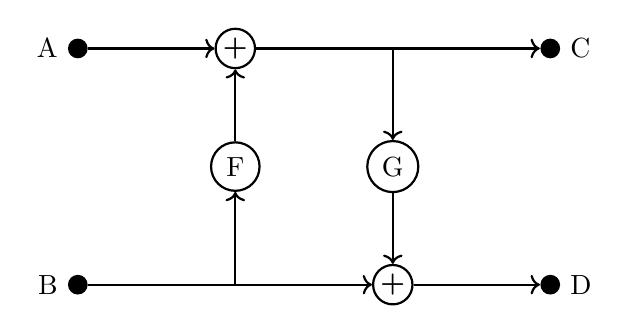
\begin{tikzpicture}[
                dot/.style = {circle, fill, inner sep = 0mm, minimum size = 2.5mm},
                op/.style = {draw, thick, circle, inner sep = 0mm, minimum size = 5mm},
                func/.style = {draw, thick, circle, inner sep = 1mm},
                arr/.style = {draw, thick, ->},
            ]
            \node (A) at (0, 3) [dot, label = left:A] {};
            \node (B) at (0, 0) [dot, label = left:B] {};
            \node (C) at (6, 3) [dot, label = right:C] {};
            \node (D) at (6, 0) [dot, label = right:D] {};

            \node (P1) at (2, 3) [op] {\textbf{+}};
            \node (P2) at (4, 0) [op] {\textbf{+}};

            \node (F) at (2, 1.5) [func] {F};
            \node (G) at (4, 1.5) [func] {G};

            \path[arr] (A) -- (P1);
            \path[arr] (P1) -- (C);
            \path[arr] (B) -- (P2);
            \path[arr] (P2) -- (D);
            \path[arr] (2, 0) -- (F);
            \path[arr] (F) -- (P1);
            \path[arr] (4, 3) -- (G);
            \path[arr] (G) -- (P2);
        \end{tikzpicture}
        \caption{Lifting steps.}
    \end{subfigure}
    \begin{subfigure}[b]{0.5\textwidth}
        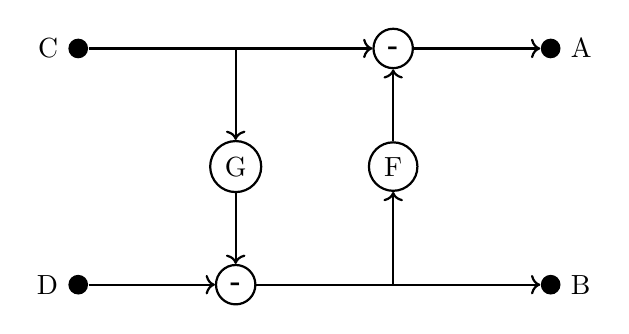
\begin{tikzpicture}[
                dot/.style = {circle, fill, inner sep = 0mm, minimum size = 2.5mm},
                op/.style = {draw, thick, circle, inner sep = 0mm, minimum size = 5mm},
                func/.style = {draw, thick, circle, inner sep = 1mm},
                arr/.style = {draw, thick, ->},
            ]
            \node (A) at (14, 3) [dot, label = right:A] {};
            \node (B) at (14, 0) [dot, label = right:B] {};
            \node (C) at (8, 3) [dot, label = left:C] {};
            \node (D) at (8, 0) [dot, label = left:D] {};

            \node (P1) at (12, 3) [op] {\textbf{-}};
            \node (P2) at (10, 0) [op] {\textbf{-}};

            \node (F) at (12, 1.5) [func] {F};
            \node (G) at (10, 1.5) [func] {G};

            \path[arr] (P1) -- (A);
            \path[arr] (C) -- (P1);
            \path[arr] (P2) -- (B);
            \path[arr] (D) -- (P2);

            \path[arr] (12, 0) -- (F);
            \path[arr] (10, 3) -- (G);
            \path[arr] (F) -- (P1);
            \path[arr] (G) -- (P2);
        \end{tikzpicture}
        \caption{Inverse path.}
    \end{subfigure}
    \caption{Dataflow path of a lifting step and its derived inverse.\label{fig:lift}}
\end{figure}

\subsection{Complex multiplication}
\begin{figure}
    \begin{subfigure}[b]{0.5\textwidth}
        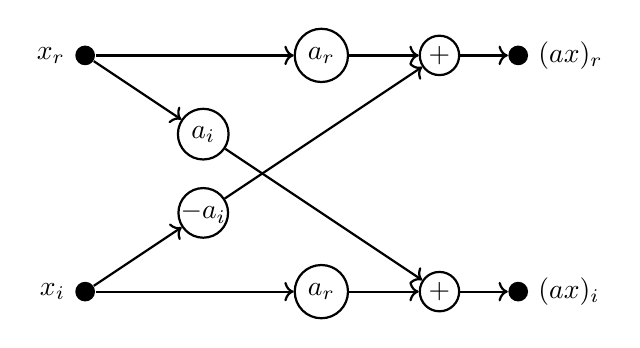
\begin{tikzpicture}[
                dot/.style = {circle, fill, inner sep = 0mm, minimum size = 2.5mm},
                op/.style = {draw, thick, circle, inner sep = 0mm, minimum size = 5mm},
                func/.style = {draw, thick, circle, inner sep = 1mm},
                arr/.style = {draw, thick, ->},
            ]
            \node (XR) [dot, label=left:$x_r$] at (0,3){};
            \node (XI) [dot, label=left:$x_i$] at (0,0){};
            \node (AXR) [dot, label=right:$(ax)_r$] at (5.5,3){};
            \node (AXI) [dot, label=right:$(ax)_i$] at (5.5,0){};

            \node (P1) [op] at (4.5, 3) {+};
            \node (P2) [op] at (4.5, 0) {+};
            \node (AR1) [func] at (3.0, 3) {$a_r$};
            \node (AR2) [func] at (3.0, 0) {$a_r$};

            \node (AI1) [func] at (1.5, 2) {$a_i$};
            \node (AI2) [op] at (1.5, 1) {$-a_i$};

            \path[arr] (XR) -- (AR1);
            \path[arr] (AR1) -- (P1);
            \path[arr] (P1) -- (AXR);

            \path[arr] (XI) -- (AR2);
            \path[arr] (AR2) -- (P2);
            \path[arr] (P2) -- (AXI);

            \path[arr] (XR) -- (AI1);
            \path[arr] (AI1) -- (P2);

            \path[arr] (XI) -- (AI2);
            \path[arr] (AI2) -- (P1);
        \end{tikzpicture}
        \caption{Butterfly structure.\label{fig:complexmula}}
    \end{subfigure}
    \begin{subfigure}[b]{0.5\textwidth}
        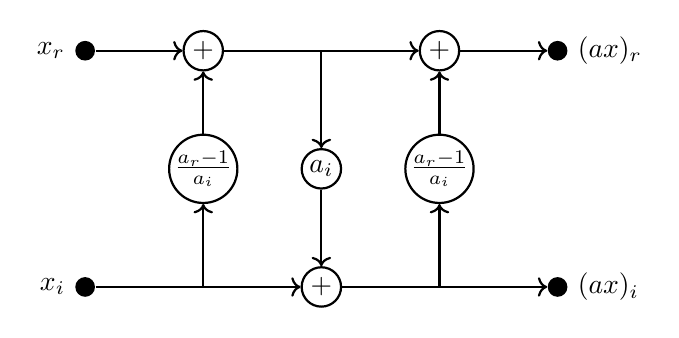
\begin{tikzpicture}[
                dot/.style = {circle, fill, inner sep = 0mm, minimum size = 2.5mm},
                op/.style = {draw, thick, circle, inner sep = 0mm, minimum size = 5mm},
                func/.style = {draw, thick, circle, inner sep = 1mm},
                arr/.style = {draw, thick, ->},
            ]
            \node (xr) [dot, label=left:$x_r$] at (0,3){};
            \node (xi) [dot, label=left:$x_i$] at (0,0){};
            \node (axr) [dot, label=right:$(ax)_r$] at (6,3){};
            \node (axi) [dot, label=right:$(ax)_i$] at (6,0){};

            \node (one) [op] at (1.5, 1.5) {$\frac{a_r - 1}{a_i}$};
            \node (two) [op] at (3, 1.5) {$a_i$};
            \node (three) [op] at (4.5, 1.5) {$\frac{a_r - 1}{a_i}$};

            \node (p1) [op] at (1.5, 3){+};
            \node (p2) [op] at (3, 0){+};
            \node (p3) [op] at (4.5, 3){+};

            \path[arr] (xr) -- (p1);
            \path[arr] (p1) -- (p3);
            \path[arr] (p3) -- (axr);

            \path[arr] (xi) -- (p2);
            \path[arr] (p2) -- (axi);

            \path[arr] (1.5, 0) -- (one);
            \path[arr] (one) -- (p1);

            \path[arr] (3, 3) -- (two);
            \path[arr] (two) -- (p2);

            \path[arr] (4.5, 0) -- (three);
            \path[arr] (three) -- (p3);
        \end{tikzpicture}
        \caption{Alternative lifting steps.\label{fig:complexmulb}}
    \end{subfigure}
    \caption{Datapaths for complex multiplication.\label{fig:complexmul}}
\end{figure}

\subsection{Reversible convolution}
\begin{figure}
    \centering
    \begin{subfigure}[b]{0.496\textwidth}
        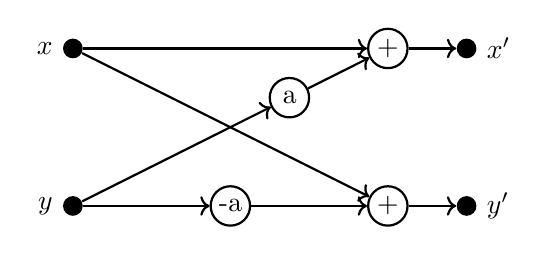
\begin{tikzpicture}[
                dot/.style = {circle, fill, inner sep = 0mm, minimum size = 2.5mm},
                op/.style = {draw, thick, circle, inner sep = 0mm, minimum size = 5mm},
                func/.style = {draw, thick, circle, inner sep = 1mm},
                arr/.style = {draw, thick, ->},
            ]
            \node (x) [dot, label=left:$x$] at (0,2){};
            \node (y) [dot, label=left:$y$] at (0,0){};
            \node (xp) [dot, label=right:$x'$] at (5,2){};
            \node (yp) [dot, label=right:$y'$] at (5,0){};

            \node (a1) [op] at (2.75, 1.375) {a};
            \node (a2) [op] at (2, 0) {-a};
            \node (p1) [op] at (4, 2) {+};
            \node (p2) [op] at (4, 0) {+};

            \path[arr] (x) -- (p1);
            \path[arr] (p1) -- (xp);
            \path[arr] (y) -- (a2);
            \path[arr] (a2) -- (p2);
            \path[arr] (p2) -- (yp);

            \path[arr] (x) -- (p2);

            \path[arr] (y) -- (a1);
            \path[arr] (a1) -- (p1);
        \end{tikzpicture}
        \caption{Butterfly structure.\label{fig:conva}}
    \end{subfigure}
    \begin{subfigure}[b]{0.496\textwidth}
        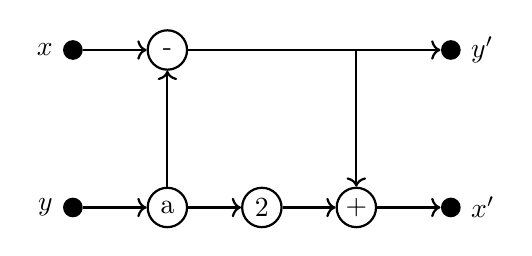
\begin{tikzpicture}[
                dot/.style = {circle, fill, inner sep = 0mm, minimum size = 2.5mm},
                op/.style = {draw, thick, circle, inner sep = 0mm, minimum size = 5mm},
                func/.style = {draw, thick, circle, inner sep = 1mm},
                arr/.style = {draw, thick, ->},
            ]
            \node (x) [dot, label=left:$x$] at (0,2){};
            \node (y) [dot, label=left:$y$] at (0,0){};
            \node (yp) [dot, label=right:$y'$] at (4.8,2){};
            \node (xp) [dot, label=right:$x'$] at (4.8,0){};

            \node (a) [op] at (1.2,0){a};
            \node (t) [op] at (2.4,0){2};
            \node (m) [op] at (1.2,2){-};
            \node (p) [op] at (3.6,0){+};

            \path[arr] (x) -- (m);
            \path[arr] (m) -- (yp);
            \path[arr] (y) -- (a);
            \path[arr] (a) -- (m);
            \path[arr] (a) -- (t);
            \path[arr] (t) -- (p);
            \path[arr] (p) -- (xp);
            \path[arr] (3.6,2) -- (p);
        \end{tikzpicture}
        \caption{Alternative lifting steps.\label{fig:convb}}
    \end{subfigure}
    \caption{Datapaths for FFT convolution.\label{fig:conv}}
\end{figure}

\begin{lstlisting}
procedure mul2
    if y = 0 then
        y += x
        x += y
        y -= x / 2
    fi y = 0
\end{lstlisting}

% TODO: Mention that the paper doesn't actually try to make directly reversible convolution

\begin{lstlisting}
x -= y
call mul2
y += x
x <=> y
\end{lstlisting}

    \section{Implementation}
Putting the theory into practice,
let us implement our algorithm in a reversible system.
Our language of choice is the extended version\cite{extjanus} of Janus\cite{janus2007}.
The extra features provided make managing a larger program much easier
than it would've been in base Janus.

Despite the lack of documentation and downloadable executables,
it was possible to implement and run the algorithm.
The code is included in appendix \ref{app:code}.
As can be seen in figure \ref{fig:test},
the program successfully computes the FFT of an input signal.
The test signal is a combination of two sine curves with different frequencies,
and the FFT is shown to clearly identify these.

Complex numbers are represented by arrays of 2 elements each.
Two arrays are used for the real and imaginary components of the main storage and twiddle factors.
To simplify things, numerical operations for complex numbers are implemented as procedures.
From there, functions for scrambling,
twiddle factor multiplication, and convolution are implemented.
The \texttt{fft} and \texttt{step} procedures manage the scrambling, multiplication, and convolving
of the array.

The bit depth of the twiddle factor was chosen somewhat arbitrarily to be 16.
The depth of the input is up to the user,
but 16 bits was chosen for the test.
This seems fitting, as most sound is stored in a signed 16 bit format.

\begin{figure}
    \centering
    \begin{subfigure}[b]{0.8\textwidth}
        \resizebox{\textwidth}{!}{%% Creator: Matplotlib, PGF backend
%%
%% To include the figure in your LaTeX document, write
%%   \input{<filename>.pgf}
%%
%% Make sure the required packages are loaded in your preamble
%%   \usepackage{pgf}
%%
%% Also ensure that all the required font packages are loaded; for instance,
%% the lmodern package is sometimes necessary when using math font.
%%   \usepackage{lmodern}
%%
%% Figures using additional raster images can only be included by \input if
%% they are in the same directory as the main LaTeX file. For loading figures
%% from other directories you can use the `import` package
%%   \usepackage{import}
%%
%% and then include the figures with
%%   \import{<path to file>}{<filename>.pgf}
%%
%% Matplotlib used the following preamble
%%   \usepackage{fontspec}
%%   \setmainfont{DejaVuSerif.ttf}[Path=\detokenize{/usr/lib/python3.10/site-packages/matplotlib/mpl-data/fonts/ttf/}]
%%   \setsansfont{DejaVuSans.ttf}[Path=\detokenize{/usr/lib/python3.10/site-packages/matplotlib/mpl-data/fonts/ttf/}]
%%   \setmonofont{DejaVuSansMono.ttf}[Path=\detokenize{/usr/lib/python3.10/site-packages/matplotlib/mpl-data/fonts/ttf/}]
%%
\begingroup%
\makeatletter%
\begin{pgfpicture}%
\pgfpathrectangle{\pgfpointorigin}{\pgfqpoint{6.400000in}{4.800000in}}%
\pgfusepath{use as bounding box, clip}%
\begin{pgfscope}%
\pgfsetbuttcap%
\pgfsetmiterjoin%
\definecolor{currentfill}{rgb}{1.000000,1.000000,1.000000}%
\pgfsetfillcolor{currentfill}%
\pgfsetlinewidth{0.000000pt}%
\definecolor{currentstroke}{rgb}{1.000000,1.000000,1.000000}%
\pgfsetstrokecolor{currentstroke}%
\pgfsetdash{}{0pt}%
\pgfpathmoveto{\pgfqpoint{0.000000in}{0.000000in}}%
\pgfpathlineto{\pgfqpoint{6.400000in}{0.000000in}}%
\pgfpathlineto{\pgfqpoint{6.400000in}{4.800000in}}%
\pgfpathlineto{\pgfqpoint{0.000000in}{4.800000in}}%
\pgfpathlineto{\pgfqpoint{0.000000in}{0.000000in}}%
\pgfpathclose%
\pgfusepath{fill}%
\end{pgfscope}%
\begin{pgfscope}%
\pgfsetbuttcap%
\pgfsetmiterjoin%
\definecolor{currentfill}{rgb}{1.000000,1.000000,1.000000}%
\pgfsetfillcolor{currentfill}%
\pgfsetlinewidth{0.000000pt}%
\definecolor{currentstroke}{rgb}{0.000000,0.000000,0.000000}%
\pgfsetstrokecolor{currentstroke}%
\pgfsetstrokeopacity{0.000000}%
\pgfsetdash{}{0pt}%
\pgfpathmoveto{\pgfqpoint{0.800000in}{0.528000in}}%
\pgfpathlineto{\pgfqpoint{5.760000in}{0.528000in}}%
\pgfpathlineto{\pgfqpoint{5.760000in}{4.224000in}}%
\pgfpathlineto{\pgfqpoint{0.800000in}{4.224000in}}%
\pgfpathlineto{\pgfqpoint{0.800000in}{0.528000in}}%
\pgfpathclose%
\pgfusepath{fill}%
\end{pgfscope}%
\begin{pgfscope}%
\pgfsetbuttcap%
\pgfsetroundjoin%
\definecolor{currentfill}{rgb}{0.000000,0.000000,0.000000}%
\pgfsetfillcolor{currentfill}%
\pgfsetlinewidth{0.803000pt}%
\definecolor{currentstroke}{rgb}{0.000000,0.000000,0.000000}%
\pgfsetstrokecolor{currentstroke}%
\pgfsetdash{}{0pt}%
\pgfsys@defobject{currentmarker}{\pgfqpoint{0.000000in}{-0.048611in}}{\pgfqpoint{0.000000in}{0.000000in}}{%
\pgfpathmoveto{\pgfqpoint{0.000000in}{0.000000in}}%
\pgfpathlineto{\pgfqpoint{0.000000in}{-0.048611in}}%
\pgfusepath{stroke,fill}%
}%
\begin{pgfscope}%
\pgfsys@transformshift{1.025455in}{0.528000in}%
\pgfsys@useobject{currentmarker}{}%
\end{pgfscope}%
\end{pgfscope}%
\begin{pgfscope}%
\definecolor{textcolor}{rgb}{0.000000,0.000000,0.000000}%
\pgfsetstrokecolor{textcolor}%
\pgfsetfillcolor{textcolor}%
\pgftext[x=1.025455in,y=0.430778in,,top]{\color{textcolor}\sffamily\fontsize{10.000000}{12.000000}\selectfont 0}%
\end{pgfscope}%
\begin{pgfscope}%
\pgfsetbuttcap%
\pgfsetroundjoin%
\definecolor{currentfill}{rgb}{0.000000,0.000000,0.000000}%
\pgfsetfillcolor{currentfill}%
\pgfsetlinewidth{0.803000pt}%
\definecolor{currentstroke}{rgb}{0.000000,0.000000,0.000000}%
\pgfsetstrokecolor{currentstroke}%
\pgfsetdash{}{0pt}%
\pgfsys@defobject{currentmarker}{\pgfqpoint{0.000000in}{-0.048611in}}{\pgfqpoint{0.000000in}{0.000000in}}{%
\pgfpathmoveto{\pgfqpoint{0.000000in}{0.000000in}}%
\pgfpathlineto{\pgfqpoint{0.000000in}{-0.048611in}}%
\pgfusepath{stroke,fill}%
}%
\begin{pgfscope}%
\pgfsys@transformshift{1.909590in}{0.528000in}%
\pgfsys@useobject{currentmarker}{}%
\end{pgfscope}%
\end{pgfscope}%
\begin{pgfscope}%
\definecolor{textcolor}{rgb}{0.000000,0.000000,0.000000}%
\pgfsetstrokecolor{textcolor}%
\pgfsetfillcolor{textcolor}%
\pgftext[x=1.909590in,y=0.430778in,,top]{\color{textcolor}\sffamily\fontsize{10.000000}{12.000000}\selectfont 50}%
\end{pgfscope}%
\begin{pgfscope}%
\pgfsetbuttcap%
\pgfsetroundjoin%
\definecolor{currentfill}{rgb}{0.000000,0.000000,0.000000}%
\pgfsetfillcolor{currentfill}%
\pgfsetlinewidth{0.803000pt}%
\definecolor{currentstroke}{rgb}{0.000000,0.000000,0.000000}%
\pgfsetstrokecolor{currentstroke}%
\pgfsetdash{}{0pt}%
\pgfsys@defobject{currentmarker}{\pgfqpoint{0.000000in}{-0.048611in}}{\pgfqpoint{0.000000in}{0.000000in}}{%
\pgfpathmoveto{\pgfqpoint{0.000000in}{0.000000in}}%
\pgfpathlineto{\pgfqpoint{0.000000in}{-0.048611in}}%
\pgfusepath{stroke,fill}%
}%
\begin{pgfscope}%
\pgfsys@transformshift{2.793725in}{0.528000in}%
\pgfsys@useobject{currentmarker}{}%
\end{pgfscope}%
\end{pgfscope}%
\begin{pgfscope}%
\definecolor{textcolor}{rgb}{0.000000,0.000000,0.000000}%
\pgfsetstrokecolor{textcolor}%
\pgfsetfillcolor{textcolor}%
\pgftext[x=2.793725in,y=0.430778in,,top]{\color{textcolor}\sffamily\fontsize{10.000000}{12.000000}\selectfont 100}%
\end{pgfscope}%
\begin{pgfscope}%
\pgfsetbuttcap%
\pgfsetroundjoin%
\definecolor{currentfill}{rgb}{0.000000,0.000000,0.000000}%
\pgfsetfillcolor{currentfill}%
\pgfsetlinewidth{0.803000pt}%
\definecolor{currentstroke}{rgb}{0.000000,0.000000,0.000000}%
\pgfsetstrokecolor{currentstroke}%
\pgfsetdash{}{0pt}%
\pgfsys@defobject{currentmarker}{\pgfqpoint{0.000000in}{-0.048611in}}{\pgfqpoint{0.000000in}{0.000000in}}{%
\pgfpathmoveto{\pgfqpoint{0.000000in}{0.000000in}}%
\pgfpathlineto{\pgfqpoint{0.000000in}{-0.048611in}}%
\pgfusepath{stroke,fill}%
}%
\begin{pgfscope}%
\pgfsys@transformshift{3.677861in}{0.528000in}%
\pgfsys@useobject{currentmarker}{}%
\end{pgfscope}%
\end{pgfscope}%
\begin{pgfscope}%
\definecolor{textcolor}{rgb}{0.000000,0.000000,0.000000}%
\pgfsetstrokecolor{textcolor}%
\pgfsetfillcolor{textcolor}%
\pgftext[x=3.677861in,y=0.430778in,,top]{\color{textcolor}\sffamily\fontsize{10.000000}{12.000000}\selectfont 150}%
\end{pgfscope}%
\begin{pgfscope}%
\pgfsetbuttcap%
\pgfsetroundjoin%
\definecolor{currentfill}{rgb}{0.000000,0.000000,0.000000}%
\pgfsetfillcolor{currentfill}%
\pgfsetlinewidth{0.803000pt}%
\definecolor{currentstroke}{rgb}{0.000000,0.000000,0.000000}%
\pgfsetstrokecolor{currentstroke}%
\pgfsetdash{}{0pt}%
\pgfsys@defobject{currentmarker}{\pgfqpoint{0.000000in}{-0.048611in}}{\pgfqpoint{0.000000in}{0.000000in}}{%
\pgfpathmoveto{\pgfqpoint{0.000000in}{0.000000in}}%
\pgfpathlineto{\pgfqpoint{0.000000in}{-0.048611in}}%
\pgfusepath{stroke,fill}%
}%
\begin{pgfscope}%
\pgfsys@transformshift{4.561996in}{0.528000in}%
\pgfsys@useobject{currentmarker}{}%
\end{pgfscope}%
\end{pgfscope}%
\begin{pgfscope}%
\definecolor{textcolor}{rgb}{0.000000,0.000000,0.000000}%
\pgfsetstrokecolor{textcolor}%
\pgfsetfillcolor{textcolor}%
\pgftext[x=4.561996in,y=0.430778in,,top]{\color{textcolor}\sffamily\fontsize{10.000000}{12.000000}\selectfont 200}%
\end{pgfscope}%
\begin{pgfscope}%
\pgfsetbuttcap%
\pgfsetroundjoin%
\definecolor{currentfill}{rgb}{0.000000,0.000000,0.000000}%
\pgfsetfillcolor{currentfill}%
\pgfsetlinewidth{0.803000pt}%
\definecolor{currentstroke}{rgb}{0.000000,0.000000,0.000000}%
\pgfsetstrokecolor{currentstroke}%
\pgfsetdash{}{0pt}%
\pgfsys@defobject{currentmarker}{\pgfqpoint{0.000000in}{-0.048611in}}{\pgfqpoint{0.000000in}{0.000000in}}{%
\pgfpathmoveto{\pgfqpoint{0.000000in}{0.000000in}}%
\pgfpathlineto{\pgfqpoint{0.000000in}{-0.048611in}}%
\pgfusepath{stroke,fill}%
}%
\begin{pgfscope}%
\pgfsys@transformshift{5.446132in}{0.528000in}%
\pgfsys@useobject{currentmarker}{}%
\end{pgfscope}%
\end{pgfscope}%
\begin{pgfscope}%
\definecolor{textcolor}{rgb}{0.000000,0.000000,0.000000}%
\pgfsetstrokecolor{textcolor}%
\pgfsetfillcolor{textcolor}%
\pgftext[x=5.446132in,y=0.430778in,,top]{\color{textcolor}\sffamily\fontsize{10.000000}{12.000000}\selectfont 250}%
\end{pgfscope}%
\begin{pgfscope}%
\definecolor{textcolor}{rgb}{0.000000,0.000000,0.000000}%
\pgfsetstrokecolor{textcolor}%
\pgfsetfillcolor{textcolor}%
\pgftext[x=3.280000in,y=0.240809in,,top]{\color{textcolor}\sffamily\fontsize{10.000000}{12.000000}\selectfont Time}%
\end{pgfscope}%
\begin{pgfscope}%
\pgfsetbuttcap%
\pgfsetroundjoin%
\definecolor{currentfill}{rgb}{0.000000,0.000000,0.000000}%
\pgfsetfillcolor{currentfill}%
\pgfsetlinewidth{0.803000pt}%
\definecolor{currentstroke}{rgb}{0.000000,0.000000,0.000000}%
\pgfsetstrokecolor{currentstroke}%
\pgfsetdash{}{0pt}%
\pgfsys@defobject{currentmarker}{\pgfqpoint{-0.048611in}{0.000000in}}{\pgfqpoint{-0.000000in}{0.000000in}}{%
\pgfpathmoveto{\pgfqpoint{-0.000000in}{0.000000in}}%
\pgfpathlineto{\pgfqpoint{-0.048611in}{0.000000in}}%
\pgfusepath{stroke,fill}%
}%
\begin{pgfscope}%
\pgfsys@transformshift{0.800000in}{0.983533in}%
\pgfsys@useobject{currentmarker}{}%
\end{pgfscope}%
\end{pgfscope}%
\begin{pgfscope}%
\definecolor{textcolor}{rgb}{0.000000,0.000000,0.000000}%
\pgfsetstrokecolor{textcolor}%
\pgfsetfillcolor{textcolor}%
\pgftext[x=0.064561in, y=0.930772in, left, base]{\color{textcolor}\sffamily\fontsize{10.000000}{12.000000}\selectfont \ensuremath{-}100000}%
\end{pgfscope}%
\begin{pgfscope}%
\pgfsetbuttcap%
\pgfsetroundjoin%
\definecolor{currentfill}{rgb}{0.000000,0.000000,0.000000}%
\pgfsetfillcolor{currentfill}%
\pgfsetlinewidth{0.803000pt}%
\definecolor{currentstroke}{rgb}{0.000000,0.000000,0.000000}%
\pgfsetstrokecolor{currentstroke}%
\pgfsetdash{}{0pt}%
\pgfsys@defobject{currentmarker}{\pgfqpoint{-0.048611in}{0.000000in}}{\pgfqpoint{-0.000000in}{0.000000in}}{%
\pgfpathmoveto{\pgfqpoint{-0.000000in}{0.000000in}}%
\pgfpathlineto{\pgfqpoint{-0.048611in}{0.000000in}}%
\pgfusepath{stroke,fill}%
}%
\begin{pgfscope}%
\pgfsys@transformshift{0.800000in}{1.679774in}%
\pgfsys@useobject{currentmarker}{}%
\end{pgfscope}%
\end{pgfscope}%
\begin{pgfscope}%
\definecolor{textcolor}{rgb}{0.000000,0.000000,0.000000}%
\pgfsetstrokecolor{textcolor}%
\pgfsetfillcolor{textcolor}%
\pgftext[x=0.152926in, y=1.627012in, left, base]{\color{textcolor}\sffamily\fontsize{10.000000}{12.000000}\selectfont \ensuremath{-}50000}%
\end{pgfscope}%
\begin{pgfscope}%
\pgfsetbuttcap%
\pgfsetroundjoin%
\definecolor{currentfill}{rgb}{0.000000,0.000000,0.000000}%
\pgfsetfillcolor{currentfill}%
\pgfsetlinewidth{0.803000pt}%
\definecolor{currentstroke}{rgb}{0.000000,0.000000,0.000000}%
\pgfsetstrokecolor{currentstroke}%
\pgfsetdash{}{0pt}%
\pgfsys@defobject{currentmarker}{\pgfqpoint{-0.048611in}{0.000000in}}{\pgfqpoint{-0.000000in}{0.000000in}}{%
\pgfpathmoveto{\pgfqpoint{-0.000000in}{0.000000in}}%
\pgfpathlineto{\pgfqpoint{-0.048611in}{0.000000in}}%
\pgfusepath{stroke,fill}%
}%
\begin{pgfscope}%
\pgfsys@transformshift{0.800000in}{2.376014in}%
\pgfsys@useobject{currentmarker}{}%
\end{pgfscope}%
\end{pgfscope}%
\begin{pgfscope}%
\definecolor{textcolor}{rgb}{0.000000,0.000000,0.000000}%
\pgfsetstrokecolor{textcolor}%
\pgfsetfillcolor{textcolor}%
\pgftext[x=0.614412in, y=2.323252in, left, base]{\color{textcolor}\sffamily\fontsize{10.000000}{12.000000}\selectfont 0}%
\end{pgfscope}%
\begin{pgfscope}%
\pgfsetbuttcap%
\pgfsetroundjoin%
\definecolor{currentfill}{rgb}{0.000000,0.000000,0.000000}%
\pgfsetfillcolor{currentfill}%
\pgfsetlinewidth{0.803000pt}%
\definecolor{currentstroke}{rgb}{0.000000,0.000000,0.000000}%
\pgfsetstrokecolor{currentstroke}%
\pgfsetdash{}{0pt}%
\pgfsys@defobject{currentmarker}{\pgfqpoint{-0.048611in}{0.000000in}}{\pgfqpoint{-0.000000in}{0.000000in}}{%
\pgfpathmoveto{\pgfqpoint{-0.000000in}{0.000000in}}%
\pgfpathlineto{\pgfqpoint{-0.048611in}{0.000000in}}%
\pgfusepath{stroke,fill}%
}%
\begin{pgfscope}%
\pgfsys@transformshift{0.800000in}{3.072254in}%
\pgfsys@useobject{currentmarker}{}%
\end{pgfscope}%
\end{pgfscope}%
\begin{pgfscope}%
\definecolor{textcolor}{rgb}{0.000000,0.000000,0.000000}%
\pgfsetstrokecolor{textcolor}%
\pgfsetfillcolor{textcolor}%
\pgftext[x=0.260951in, y=3.019493in, left, base]{\color{textcolor}\sffamily\fontsize{10.000000}{12.000000}\selectfont 50000}%
\end{pgfscope}%
\begin{pgfscope}%
\pgfsetbuttcap%
\pgfsetroundjoin%
\definecolor{currentfill}{rgb}{0.000000,0.000000,0.000000}%
\pgfsetfillcolor{currentfill}%
\pgfsetlinewidth{0.803000pt}%
\definecolor{currentstroke}{rgb}{0.000000,0.000000,0.000000}%
\pgfsetstrokecolor{currentstroke}%
\pgfsetdash{}{0pt}%
\pgfsys@defobject{currentmarker}{\pgfqpoint{-0.048611in}{0.000000in}}{\pgfqpoint{-0.000000in}{0.000000in}}{%
\pgfpathmoveto{\pgfqpoint{-0.000000in}{0.000000in}}%
\pgfpathlineto{\pgfqpoint{-0.048611in}{0.000000in}}%
\pgfusepath{stroke,fill}%
}%
\begin{pgfscope}%
\pgfsys@transformshift{0.800000in}{3.768495in}%
\pgfsys@useobject{currentmarker}{}%
\end{pgfscope}%
\end{pgfscope}%
\begin{pgfscope}%
\definecolor{textcolor}{rgb}{0.000000,0.000000,0.000000}%
\pgfsetstrokecolor{textcolor}%
\pgfsetfillcolor{textcolor}%
\pgftext[x=0.172586in, y=3.715733in, left, base]{\color{textcolor}\sffamily\fontsize{10.000000}{12.000000}\selectfont 100000}%
\end{pgfscope}%
\begin{pgfscope}%
\definecolor{textcolor}{rgb}{0.000000,0.000000,0.000000}%
\pgfsetstrokecolor{textcolor}%
\pgfsetfillcolor{textcolor}%
\pgftext[x=0.009005in,y=2.376000in,,bottom,rotate=90.000000]{\color{textcolor}\sffamily\fontsize{10.000000}{12.000000}\selectfont Strength}%
\end{pgfscope}%
\begin{pgfscope}%
\pgfpathrectangle{\pgfqpoint{0.800000in}{0.528000in}}{\pgfqpoint{4.960000in}{3.696000in}}%
\pgfusepath{clip}%
\pgfsetrectcap%
\pgfsetroundjoin%
\pgfsetlinewidth{1.505625pt}%
\definecolor{currentstroke}{rgb}{0.121569,0.466667,0.705882}%
\pgfsetstrokecolor{currentstroke}%
\pgfsetdash{}{0pt}%
\pgfpathmoveto{\pgfqpoint{1.025455in}{2.376014in}}%
\pgfpathlineto{\pgfqpoint{1.043137in}{3.879796in}}%
\pgfpathlineto{\pgfqpoint{1.060820in}{2.475381in}}%
\pgfpathlineto{\pgfqpoint{1.078503in}{2.771952in}}%
\pgfpathlineto{\pgfqpoint{1.096185in}{2.770351in}}%
\pgfpathlineto{\pgfqpoint{1.113868in}{0.696000in}}%
\pgfpathlineto{\pgfqpoint{1.131551in}{1.662507in}}%
\pgfpathlineto{\pgfqpoint{1.149234in}{3.166302in}}%
\pgfpathlineto{\pgfqpoint{1.166916in}{2.299177in}}%
\pgfpathlineto{\pgfqpoint{1.184599in}{3.265684in}}%
\pgfpathlineto{\pgfqpoint{1.202282in}{3.562268in}}%
\pgfpathlineto{\pgfqpoint{1.219964in}{1.189732in}}%
\pgfpathlineto{\pgfqpoint{1.237647in}{1.486302in}}%
\pgfpathlineto{\pgfqpoint{1.255330in}{2.452823in}}%
\pgfpathlineto{\pgfqpoint{1.273012in}{1.585684in}}%
\pgfpathlineto{\pgfqpoint{1.290695in}{3.089479in}}%
\pgfpathlineto{\pgfqpoint{1.308378in}{4.056000in}}%
\pgfpathlineto{\pgfqpoint{1.326061in}{1.981649in}}%
\pgfpathlineto{\pgfqpoint{1.343743in}{1.980034in}}%
\pgfpathlineto{\pgfqpoint{1.361426in}{2.276619in}}%
\pgfpathlineto{\pgfqpoint{1.379109in}{0.872204in}}%
\pgfpathlineto{\pgfqpoint{1.414474in}{3.879796in}}%
\pgfpathlineto{\pgfqpoint{1.432157in}{2.475381in}}%
\pgfpathlineto{\pgfqpoint{1.449840in}{2.771952in}}%
\pgfpathlineto{\pgfqpoint{1.467522in}{2.770351in}}%
\pgfpathlineto{\pgfqpoint{1.485205in}{0.696000in}}%
\pgfpathlineto{\pgfqpoint{1.502888in}{1.662507in}}%
\pgfpathlineto{\pgfqpoint{1.520570in}{3.166302in}}%
\pgfpathlineto{\pgfqpoint{1.538253in}{2.299177in}}%
\pgfpathlineto{\pgfqpoint{1.555936in}{3.265684in}}%
\pgfpathlineto{\pgfqpoint{1.573619in}{3.562268in}}%
\pgfpathlineto{\pgfqpoint{1.591301in}{1.189732in}}%
\pgfpathlineto{\pgfqpoint{1.608984in}{1.486302in}}%
\pgfpathlineto{\pgfqpoint{1.626667in}{2.452823in}}%
\pgfpathlineto{\pgfqpoint{1.644349in}{1.585684in}}%
\pgfpathlineto{\pgfqpoint{1.662032in}{3.089479in}}%
\pgfpathlineto{\pgfqpoint{1.679715in}{4.056000in}}%
\pgfpathlineto{\pgfqpoint{1.697398in}{1.981649in}}%
\pgfpathlineto{\pgfqpoint{1.715080in}{1.980034in}}%
\pgfpathlineto{\pgfqpoint{1.732763in}{2.276619in}}%
\pgfpathlineto{\pgfqpoint{1.750446in}{0.872204in}}%
\pgfpathlineto{\pgfqpoint{1.785811in}{3.879796in}}%
\pgfpathlineto{\pgfqpoint{1.803494in}{2.475381in}}%
\pgfpathlineto{\pgfqpoint{1.821176in}{2.771952in}}%
\pgfpathlineto{\pgfqpoint{1.838859in}{2.770351in}}%
\pgfpathlineto{\pgfqpoint{1.856542in}{0.696000in}}%
\pgfpathlineto{\pgfqpoint{1.874225in}{1.662507in}}%
\pgfpathlineto{\pgfqpoint{1.891907in}{3.166302in}}%
\pgfpathlineto{\pgfqpoint{1.909590in}{2.299177in}}%
\pgfpathlineto{\pgfqpoint{1.927273in}{3.265684in}}%
\pgfpathlineto{\pgfqpoint{1.944955in}{3.562268in}}%
\pgfpathlineto{\pgfqpoint{1.962638in}{1.189732in}}%
\pgfpathlineto{\pgfqpoint{1.980321in}{1.486302in}}%
\pgfpathlineto{\pgfqpoint{1.998004in}{2.452823in}}%
\pgfpathlineto{\pgfqpoint{2.015686in}{1.585684in}}%
\pgfpathlineto{\pgfqpoint{2.033369in}{3.089479in}}%
\pgfpathlineto{\pgfqpoint{2.051052in}{4.056000in}}%
\pgfpathlineto{\pgfqpoint{2.068734in}{1.981649in}}%
\pgfpathlineto{\pgfqpoint{2.086417in}{1.980034in}}%
\pgfpathlineto{\pgfqpoint{2.104100in}{2.276619in}}%
\pgfpathlineto{\pgfqpoint{2.121783in}{0.872204in}}%
\pgfpathlineto{\pgfqpoint{2.157148in}{3.879796in}}%
\pgfpathlineto{\pgfqpoint{2.174831in}{2.475381in}}%
\pgfpathlineto{\pgfqpoint{2.192513in}{2.771952in}}%
\pgfpathlineto{\pgfqpoint{2.210196in}{2.770351in}}%
\pgfpathlineto{\pgfqpoint{2.227879in}{0.696000in}}%
\pgfpathlineto{\pgfqpoint{2.245561in}{1.662507in}}%
\pgfpathlineto{\pgfqpoint{2.263244in}{3.166302in}}%
\pgfpathlineto{\pgfqpoint{2.280927in}{2.299177in}}%
\pgfpathlineto{\pgfqpoint{2.298610in}{3.265684in}}%
\pgfpathlineto{\pgfqpoint{2.316292in}{3.562268in}}%
\pgfpathlineto{\pgfqpoint{2.333975in}{1.189732in}}%
\pgfpathlineto{\pgfqpoint{2.351658in}{1.486302in}}%
\pgfpathlineto{\pgfqpoint{2.369340in}{2.452823in}}%
\pgfpathlineto{\pgfqpoint{2.387023in}{1.585684in}}%
\pgfpathlineto{\pgfqpoint{2.404706in}{3.089479in}}%
\pgfpathlineto{\pgfqpoint{2.422389in}{4.056000in}}%
\pgfpathlineto{\pgfqpoint{2.440071in}{1.981649in}}%
\pgfpathlineto{\pgfqpoint{2.457754in}{1.980034in}}%
\pgfpathlineto{\pgfqpoint{2.475437in}{2.276619in}}%
\pgfpathlineto{\pgfqpoint{2.493119in}{0.872204in}}%
\pgfpathlineto{\pgfqpoint{2.528485in}{3.879796in}}%
\pgfpathlineto{\pgfqpoint{2.546168in}{2.475381in}}%
\pgfpathlineto{\pgfqpoint{2.563850in}{2.771952in}}%
\pgfpathlineto{\pgfqpoint{2.581533in}{2.770351in}}%
\pgfpathlineto{\pgfqpoint{2.599216in}{0.696000in}}%
\pgfpathlineto{\pgfqpoint{2.616898in}{1.662507in}}%
\pgfpathlineto{\pgfqpoint{2.634581in}{3.166316in}}%
\pgfpathlineto{\pgfqpoint{2.652264in}{2.299177in}}%
\pgfpathlineto{\pgfqpoint{2.669947in}{3.265684in}}%
\pgfpathlineto{\pgfqpoint{2.687629in}{3.562268in}}%
\pgfpathlineto{\pgfqpoint{2.705312in}{1.189732in}}%
\pgfpathlineto{\pgfqpoint{2.722995in}{1.486302in}}%
\pgfpathlineto{\pgfqpoint{2.740677in}{2.452823in}}%
\pgfpathlineto{\pgfqpoint{2.758360in}{1.585684in}}%
\pgfpathlineto{\pgfqpoint{2.776043in}{3.089479in}}%
\pgfpathlineto{\pgfqpoint{2.793725in}{4.056000in}}%
\pgfpathlineto{\pgfqpoint{2.811408in}{1.981649in}}%
\pgfpathlineto{\pgfqpoint{2.829091in}{1.980034in}}%
\pgfpathlineto{\pgfqpoint{2.846774in}{2.276619in}}%
\pgfpathlineto{\pgfqpoint{2.864456in}{0.872204in}}%
\pgfpathlineto{\pgfqpoint{2.899822in}{3.879796in}}%
\pgfpathlineto{\pgfqpoint{2.917504in}{2.475381in}}%
\pgfpathlineto{\pgfqpoint{2.935187in}{2.771952in}}%
\pgfpathlineto{\pgfqpoint{2.952870in}{2.770351in}}%
\pgfpathlineto{\pgfqpoint{2.970553in}{0.696000in}}%
\pgfpathlineto{\pgfqpoint{2.988235in}{1.662507in}}%
\pgfpathlineto{\pgfqpoint{3.005918in}{3.166302in}}%
\pgfpathlineto{\pgfqpoint{3.023601in}{2.299177in}}%
\pgfpathlineto{\pgfqpoint{3.041283in}{3.265684in}}%
\pgfpathlineto{\pgfqpoint{3.058966in}{3.562268in}}%
\pgfpathlineto{\pgfqpoint{3.076649in}{1.189732in}}%
\pgfpathlineto{\pgfqpoint{3.094332in}{1.486302in}}%
\pgfpathlineto{\pgfqpoint{3.112014in}{2.452823in}}%
\pgfpathlineto{\pgfqpoint{3.129697in}{1.585698in}}%
\pgfpathlineto{\pgfqpoint{3.147380in}{3.089479in}}%
\pgfpathlineto{\pgfqpoint{3.165062in}{4.056000in}}%
\pgfpathlineto{\pgfqpoint{3.182745in}{1.981649in}}%
\pgfpathlineto{\pgfqpoint{3.200428in}{1.980034in}}%
\pgfpathlineto{\pgfqpoint{3.218111in}{2.276619in}}%
\pgfpathlineto{\pgfqpoint{3.235793in}{0.872204in}}%
\pgfpathlineto{\pgfqpoint{3.271159in}{3.879796in}}%
\pgfpathlineto{\pgfqpoint{3.288841in}{2.475381in}}%
\pgfpathlineto{\pgfqpoint{3.306524in}{2.771952in}}%
\pgfpathlineto{\pgfqpoint{3.324207in}{2.770351in}}%
\pgfpathlineto{\pgfqpoint{3.341889in}{0.696000in}}%
\pgfpathlineto{\pgfqpoint{3.359572in}{1.662507in}}%
\pgfpathlineto{\pgfqpoint{3.377255in}{3.166302in}}%
\pgfpathlineto{\pgfqpoint{3.394938in}{2.299177in}}%
\pgfpathlineto{\pgfqpoint{3.412620in}{3.265684in}}%
\pgfpathlineto{\pgfqpoint{3.430303in}{3.562268in}}%
\pgfpathlineto{\pgfqpoint{3.447986in}{1.189732in}}%
\pgfpathlineto{\pgfqpoint{3.465668in}{1.486302in}}%
\pgfpathlineto{\pgfqpoint{3.483351in}{2.452823in}}%
\pgfpathlineto{\pgfqpoint{3.501034in}{1.585684in}}%
\pgfpathlineto{\pgfqpoint{3.518717in}{3.089479in}}%
\pgfpathlineto{\pgfqpoint{3.536399in}{4.056000in}}%
\pgfpathlineto{\pgfqpoint{3.554082in}{1.981649in}}%
\pgfpathlineto{\pgfqpoint{3.571765in}{1.980034in}}%
\pgfpathlineto{\pgfqpoint{3.589447in}{2.276619in}}%
\pgfpathlineto{\pgfqpoint{3.607130in}{0.872204in}}%
\pgfpathlineto{\pgfqpoint{3.642496in}{3.879796in}}%
\pgfpathlineto{\pgfqpoint{3.660178in}{2.475381in}}%
\pgfpathlineto{\pgfqpoint{3.677861in}{2.771952in}}%
\pgfpathlineto{\pgfqpoint{3.695544in}{2.770351in}}%
\pgfpathlineto{\pgfqpoint{3.713226in}{0.696000in}}%
\pgfpathlineto{\pgfqpoint{3.730909in}{1.662507in}}%
\pgfpathlineto{\pgfqpoint{3.748592in}{3.166302in}}%
\pgfpathlineto{\pgfqpoint{3.766275in}{2.299177in}}%
\pgfpathlineto{\pgfqpoint{3.783957in}{3.265684in}}%
\pgfpathlineto{\pgfqpoint{3.801640in}{3.562268in}}%
\pgfpathlineto{\pgfqpoint{3.819323in}{1.189732in}}%
\pgfpathlineto{\pgfqpoint{3.837005in}{1.486302in}}%
\pgfpathlineto{\pgfqpoint{3.854688in}{2.452823in}}%
\pgfpathlineto{\pgfqpoint{3.872371in}{1.585684in}}%
\pgfpathlineto{\pgfqpoint{3.890053in}{3.089479in}}%
\pgfpathlineto{\pgfqpoint{3.907736in}{4.056000in}}%
\pgfpathlineto{\pgfqpoint{3.925419in}{1.981649in}}%
\pgfpathlineto{\pgfqpoint{3.943102in}{1.980034in}}%
\pgfpathlineto{\pgfqpoint{3.960784in}{2.276619in}}%
\pgfpathlineto{\pgfqpoint{3.978467in}{0.872204in}}%
\pgfpathlineto{\pgfqpoint{4.013832in}{3.879796in}}%
\pgfpathlineto{\pgfqpoint{4.031515in}{2.475381in}}%
\pgfpathlineto{\pgfqpoint{4.049198in}{2.771952in}}%
\pgfpathlineto{\pgfqpoint{4.066881in}{2.770351in}}%
\pgfpathlineto{\pgfqpoint{4.084563in}{0.696000in}}%
\pgfpathlineto{\pgfqpoint{4.102246in}{1.662507in}}%
\pgfpathlineto{\pgfqpoint{4.119929in}{3.166316in}}%
\pgfpathlineto{\pgfqpoint{4.137611in}{2.299177in}}%
\pgfpathlineto{\pgfqpoint{4.155294in}{3.265684in}}%
\pgfpathlineto{\pgfqpoint{4.172977in}{3.562268in}}%
\pgfpathlineto{\pgfqpoint{4.190660in}{1.189732in}}%
\pgfpathlineto{\pgfqpoint{4.208342in}{1.486302in}}%
\pgfpathlineto{\pgfqpoint{4.226025in}{2.452823in}}%
\pgfpathlineto{\pgfqpoint{4.243708in}{1.585698in}}%
\pgfpathlineto{\pgfqpoint{4.261390in}{3.089479in}}%
\pgfpathlineto{\pgfqpoint{4.279073in}{4.056000in}}%
\pgfpathlineto{\pgfqpoint{4.296756in}{1.981649in}}%
\pgfpathlineto{\pgfqpoint{4.314439in}{1.980034in}}%
\pgfpathlineto{\pgfqpoint{4.332121in}{2.276619in}}%
\pgfpathlineto{\pgfqpoint{4.349804in}{0.872204in}}%
\pgfpathlineto{\pgfqpoint{4.385169in}{3.879796in}}%
\pgfpathlineto{\pgfqpoint{4.402852in}{2.475381in}}%
\pgfpathlineto{\pgfqpoint{4.420535in}{2.771952in}}%
\pgfpathlineto{\pgfqpoint{4.438217in}{2.770351in}}%
\pgfpathlineto{\pgfqpoint{4.455900in}{0.696000in}}%
\pgfpathlineto{\pgfqpoint{4.473583in}{1.662507in}}%
\pgfpathlineto{\pgfqpoint{4.491266in}{3.166302in}}%
\pgfpathlineto{\pgfqpoint{4.508948in}{2.299177in}}%
\pgfpathlineto{\pgfqpoint{4.526631in}{3.265684in}}%
\pgfpathlineto{\pgfqpoint{4.544314in}{3.562268in}}%
\pgfpathlineto{\pgfqpoint{4.561996in}{1.189732in}}%
\pgfpathlineto{\pgfqpoint{4.579679in}{1.486302in}}%
\pgfpathlineto{\pgfqpoint{4.597362in}{2.452823in}}%
\pgfpathlineto{\pgfqpoint{4.615045in}{1.585698in}}%
\pgfpathlineto{\pgfqpoint{4.632727in}{3.089479in}}%
\pgfpathlineto{\pgfqpoint{4.650410in}{4.056000in}}%
\pgfpathlineto{\pgfqpoint{4.668093in}{1.981649in}}%
\pgfpathlineto{\pgfqpoint{4.685775in}{1.980034in}}%
\pgfpathlineto{\pgfqpoint{4.703458in}{2.276619in}}%
\pgfpathlineto{\pgfqpoint{4.721141in}{0.872204in}}%
\pgfpathlineto{\pgfqpoint{4.756506in}{3.879796in}}%
\pgfpathlineto{\pgfqpoint{4.774189in}{2.475381in}}%
\pgfpathlineto{\pgfqpoint{4.791872in}{2.771952in}}%
\pgfpathlineto{\pgfqpoint{4.809554in}{2.770351in}}%
\pgfpathlineto{\pgfqpoint{4.827237in}{0.696000in}}%
\pgfpathlineto{\pgfqpoint{4.844920in}{1.662507in}}%
\pgfpathlineto{\pgfqpoint{4.862602in}{3.166302in}}%
\pgfpathlineto{\pgfqpoint{4.880285in}{2.299177in}}%
\pgfpathlineto{\pgfqpoint{4.897968in}{3.265684in}}%
\pgfpathlineto{\pgfqpoint{4.915651in}{3.562268in}}%
\pgfpathlineto{\pgfqpoint{4.933333in}{1.189732in}}%
\pgfpathlineto{\pgfqpoint{4.951016in}{1.486302in}}%
\pgfpathlineto{\pgfqpoint{4.968699in}{2.452823in}}%
\pgfpathlineto{\pgfqpoint{4.986381in}{1.585684in}}%
\pgfpathlineto{\pgfqpoint{5.004064in}{3.089479in}}%
\pgfpathlineto{\pgfqpoint{5.021747in}{4.056000in}}%
\pgfpathlineto{\pgfqpoint{5.039430in}{1.981649in}}%
\pgfpathlineto{\pgfqpoint{5.057112in}{1.980034in}}%
\pgfpathlineto{\pgfqpoint{5.074795in}{2.276619in}}%
\pgfpathlineto{\pgfqpoint{5.092478in}{0.872204in}}%
\pgfpathlineto{\pgfqpoint{5.127843in}{3.879796in}}%
\pgfpathlineto{\pgfqpoint{5.145526in}{2.475381in}}%
\pgfpathlineto{\pgfqpoint{5.163209in}{2.771952in}}%
\pgfpathlineto{\pgfqpoint{5.180891in}{2.770351in}}%
\pgfpathlineto{\pgfqpoint{5.198574in}{0.696000in}}%
\pgfpathlineto{\pgfqpoint{5.216257in}{1.662507in}}%
\pgfpathlineto{\pgfqpoint{5.233939in}{3.166316in}}%
\pgfpathlineto{\pgfqpoint{5.251622in}{2.299177in}}%
\pgfpathlineto{\pgfqpoint{5.269305in}{3.265684in}}%
\pgfpathlineto{\pgfqpoint{5.286988in}{3.562268in}}%
\pgfpathlineto{\pgfqpoint{5.304670in}{1.189732in}}%
\pgfpathlineto{\pgfqpoint{5.322353in}{1.486302in}}%
\pgfpathlineto{\pgfqpoint{5.340036in}{2.452823in}}%
\pgfpathlineto{\pgfqpoint{5.357718in}{1.585684in}}%
\pgfpathlineto{\pgfqpoint{5.375401in}{3.089479in}}%
\pgfpathlineto{\pgfqpoint{5.393084in}{4.056000in}}%
\pgfpathlineto{\pgfqpoint{5.410766in}{1.981649in}}%
\pgfpathlineto{\pgfqpoint{5.428449in}{1.980034in}}%
\pgfpathlineto{\pgfqpoint{5.446132in}{2.276619in}}%
\pgfpathlineto{\pgfqpoint{5.463815in}{0.872204in}}%
\pgfpathlineto{\pgfqpoint{5.499180in}{3.879796in}}%
\pgfpathlineto{\pgfqpoint{5.516863in}{2.475381in}}%
\pgfpathlineto{\pgfqpoint{5.534545in}{2.771952in}}%
\pgfpathlineto{\pgfqpoint{5.534545in}{2.771952in}}%
\pgfusepath{stroke}%
\end{pgfscope}%
\begin{pgfscope}%
\pgfsetrectcap%
\pgfsetmiterjoin%
\pgfsetlinewidth{0.803000pt}%
\definecolor{currentstroke}{rgb}{0.000000,0.000000,0.000000}%
\pgfsetstrokecolor{currentstroke}%
\pgfsetdash{}{0pt}%
\pgfpathmoveto{\pgfqpoint{0.800000in}{0.528000in}}%
\pgfpathlineto{\pgfqpoint{0.800000in}{4.224000in}}%
\pgfusepath{stroke}%
\end{pgfscope}%
\begin{pgfscope}%
\pgfsetrectcap%
\pgfsetmiterjoin%
\pgfsetlinewidth{0.803000pt}%
\definecolor{currentstroke}{rgb}{0.000000,0.000000,0.000000}%
\pgfsetstrokecolor{currentstroke}%
\pgfsetdash{}{0pt}%
\pgfpathmoveto{\pgfqpoint{5.760000in}{0.528000in}}%
\pgfpathlineto{\pgfqpoint{5.760000in}{4.224000in}}%
\pgfusepath{stroke}%
\end{pgfscope}%
\begin{pgfscope}%
\pgfsetrectcap%
\pgfsetmiterjoin%
\pgfsetlinewidth{0.803000pt}%
\definecolor{currentstroke}{rgb}{0.000000,0.000000,0.000000}%
\pgfsetstrokecolor{currentstroke}%
\pgfsetdash{}{0pt}%
\pgfpathmoveto{\pgfqpoint{0.800000in}{0.528000in}}%
\pgfpathlineto{\pgfqpoint{5.760000in}{0.528000in}}%
\pgfusepath{stroke}%
\end{pgfscope}%
\begin{pgfscope}%
\pgfsetrectcap%
\pgfsetmiterjoin%
\pgfsetlinewidth{0.803000pt}%
\definecolor{currentstroke}{rgb}{0.000000,0.000000,0.000000}%
\pgfsetstrokecolor{currentstroke}%
\pgfsetdash{}{0pt}%
\pgfpathmoveto{\pgfqpoint{0.800000in}{4.224000in}}%
\pgfpathlineto{\pgfqpoint{5.760000in}{4.224000in}}%
\pgfusepath{stroke}%
\end{pgfscope}%
\end{pgfpicture}%
\makeatother%
\endgroup%
}
        \caption{Input signal: two combined sine functions with frequencies $1/3$ and $1/7$.}
    \end{subfigure}
    \begin{subfigure}[b]{0.8\textwidth}
        \resizebox{\textwidth}{!}{%% Creator: Matplotlib, PGF backend
%%
%% To include the figure in your LaTeX document, write
%%   \input{<filename>.pgf}
%%
%% Make sure the required packages are loaded in your preamble
%%   \usepackage{pgf}
%%
%% Also ensure that all the required font packages are loaded; for instance,
%% the lmodern package is sometimes necessary when using math font.
%%   \usepackage{lmodern}
%%
%% Figures using additional raster images can only be included by \input if
%% they are in the same directory as the main LaTeX file. For loading figures
%% from other directories you can use the `import` package
%%   \usepackage{import}
%%
%% and then include the figures with
%%   \import{<path to file>}{<filename>.pgf}
%%
%% Matplotlib used the following preamble
%%   \usepackage{fontspec}
%%   \setmainfont{DejaVuSerif.ttf}[Path=\detokenize{/usr/lib/python3.10/site-packages/matplotlib/mpl-data/fonts/ttf/}]
%%   \setsansfont{DejaVuSans.ttf}[Path=\detokenize{/usr/lib/python3.10/site-packages/matplotlib/mpl-data/fonts/ttf/}]
%%   \setmonofont{DejaVuSansMono.ttf}[Path=\detokenize{/usr/lib/python3.10/site-packages/matplotlib/mpl-data/fonts/ttf/}]
%%
\begingroup%
\makeatletter%
\begin{pgfpicture}%
\pgfpathrectangle{\pgfpointorigin}{\pgfqpoint{6.400000in}{4.800000in}}%
\pgfusepath{use as bounding box, clip}%
\begin{pgfscope}%
\pgfsetbuttcap%
\pgfsetmiterjoin%
\definecolor{currentfill}{rgb}{1.000000,1.000000,1.000000}%
\pgfsetfillcolor{currentfill}%
\pgfsetlinewidth{0.000000pt}%
\definecolor{currentstroke}{rgb}{1.000000,1.000000,1.000000}%
\pgfsetstrokecolor{currentstroke}%
\pgfsetdash{}{0pt}%
\pgfpathmoveto{\pgfqpoint{0.000000in}{0.000000in}}%
\pgfpathlineto{\pgfqpoint{6.400000in}{0.000000in}}%
\pgfpathlineto{\pgfqpoint{6.400000in}{4.800000in}}%
\pgfpathlineto{\pgfqpoint{0.000000in}{4.800000in}}%
\pgfpathlineto{\pgfqpoint{0.000000in}{0.000000in}}%
\pgfpathclose%
\pgfusepath{fill}%
\end{pgfscope}%
\begin{pgfscope}%
\pgfsetbuttcap%
\pgfsetmiterjoin%
\definecolor{currentfill}{rgb}{1.000000,1.000000,1.000000}%
\pgfsetfillcolor{currentfill}%
\pgfsetlinewidth{0.000000pt}%
\definecolor{currentstroke}{rgb}{0.000000,0.000000,0.000000}%
\pgfsetstrokecolor{currentstroke}%
\pgfsetstrokeopacity{0.000000}%
\pgfsetdash{}{0pt}%
\pgfpathmoveto{\pgfqpoint{0.800000in}{0.528000in}}%
\pgfpathlineto{\pgfqpoint{5.760000in}{0.528000in}}%
\pgfpathlineto{\pgfqpoint{5.760000in}{4.224000in}}%
\pgfpathlineto{\pgfqpoint{0.800000in}{4.224000in}}%
\pgfpathlineto{\pgfqpoint{0.800000in}{0.528000in}}%
\pgfpathclose%
\pgfusepath{fill}%
\end{pgfscope}%
\begin{pgfscope}%
\pgfsetbuttcap%
\pgfsetroundjoin%
\definecolor{currentfill}{rgb}{0.000000,0.000000,0.000000}%
\pgfsetfillcolor{currentfill}%
\pgfsetlinewidth{0.803000pt}%
\definecolor{currentstroke}{rgb}{0.000000,0.000000,0.000000}%
\pgfsetstrokecolor{currentstroke}%
\pgfsetdash{}{0pt}%
\pgfsys@defobject{currentmarker}{\pgfqpoint{0.000000in}{-0.048611in}}{\pgfqpoint{0.000000in}{0.000000in}}{%
\pgfpathmoveto{\pgfqpoint{0.000000in}{0.000000in}}%
\pgfpathlineto{\pgfqpoint{0.000000in}{-0.048611in}}%
\pgfusepath{stroke,fill}%
}%
\begin{pgfscope}%
\pgfsys@transformshift{1.025455in}{0.528000in}%
\pgfsys@useobject{currentmarker}{}%
\end{pgfscope}%
\end{pgfscope}%
\begin{pgfscope}%
\definecolor{textcolor}{rgb}{0.000000,0.000000,0.000000}%
\pgfsetstrokecolor{textcolor}%
\pgfsetfillcolor{textcolor}%
\pgftext[x=1.025455in,y=0.430778in,,top]{\color{textcolor}\sffamily\fontsize{10.000000}{12.000000}\selectfont 0}%
\end{pgfscope}%
\begin{pgfscope}%
\pgfsetbuttcap%
\pgfsetroundjoin%
\definecolor{currentfill}{rgb}{0.000000,0.000000,0.000000}%
\pgfsetfillcolor{currentfill}%
\pgfsetlinewidth{0.803000pt}%
\definecolor{currentstroke}{rgb}{0.000000,0.000000,0.000000}%
\pgfsetstrokecolor{currentstroke}%
\pgfsetdash{}{0pt}%
\pgfsys@defobject{currentmarker}{\pgfqpoint{0.000000in}{-0.048611in}}{\pgfqpoint{0.000000in}{0.000000in}}{%
\pgfpathmoveto{\pgfqpoint{0.000000in}{0.000000in}}%
\pgfpathlineto{\pgfqpoint{0.000000in}{-0.048611in}}%
\pgfusepath{stroke,fill}%
}%
\begin{pgfscope}%
\pgfsys@transformshift{1.909590in}{0.528000in}%
\pgfsys@useobject{currentmarker}{}%
\end{pgfscope}%
\end{pgfscope}%
\begin{pgfscope}%
\definecolor{textcolor}{rgb}{0.000000,0.000000,0.000000}%
\pgfsetstrokecolor{textcolor}%
\pgfsetfillcolor{textcolor}%
\pgftext[x=1.909590in,y=0.430778in,,top]{\color{textcolor}\sffamily\fontsize{10.000000}{12.000000}\selectfont 50}%
\end{pgfscope}%
\begin{pgfscope}%
\pgfsetbuttcap%
\pgfsetroundjoin%
\definecolor{currentfill}{rgb}{0.000000,0.000000,0.000000}%
\pgfsetfillcolor{currentfill}%
\pgfsetlinewidth{0.803000pt}%
\definecolor{currentstroke}{rgb}{0.000000,0.000000,0.000000}%
\pgfsetstrokecolor{currentstroke}%
\pgfsetdash{}{0pt}%
\pgfsys@defobject{currentmarker}{\pgfqpoint{0.000000in}{-0.048611in}}{\pgfqpoint{0.000000in}{0.000000in}}{%
\pgfpathmoveto{\pgfqpoint{0.000000in}{0.000000in}}%
\pgfpathlineto{\pgfqpoint{0.000000in}{-0.048611in}}%
\pgfusepath{stroke,fill}%
}%
\begin{pgfscope}%
\pgfsys@transformshift{2.793725in}{0.528000in}%
\pgfsys@useobject{currentmarker}{}%
\end{pgfscope}%
\end{pgfscope}%
\begin{pgfscope}%
\definecolor{textcolor}{rgb}{0.000000,0.000000,0.000000}%
\pgfsetstrokecolor{textcolor}%
\pgfsetfillcolor{textcolor}%
\pgftext[x=2.793725in,y=0.430778in,,top]{\color{textcolor}\sffamily\fontsize{10.000000}{12.000000}\selectfont 100}%
\end{pgfscope}%
\begin{pgfscope}%
\pgfsetbuttcap%
\pgfsetroundjoin%
\definecolor{currentfill}{rgb}{0.000000,0.000000,0.000000}%
\pgfsetfillcolor{currentfill}%
\pgfsetlinewidth{0.803000pt}%
\definecolor{currentstroke}{rgb}{0.000000,0.000000,0.000000}%
\pgfsetstrokecolor{currentstroke}%
\pgfsetdash{}{0pt}%
\pgfsys@defobject{currentmarker}{\pgfqpoint{0.000000in}{-0.048611in}}{\pgfqpoint{0.000000in}{0.000000in}}{%
\pgfpathmoveto{\pgfqpoint{0.000000in}{0.000000in}}%
\pgfpathlineto{\pgfqpoint{0.000000in}{-0.048611in}}%
\pgfusepath{stroke,fill}%
}%
\begin{pgfscope}%
\pgfsys@transformshift{3.677861in}{0.528000in}%
\pgfsys@useobject{currentmarker}{}%
\end{pgfscope}%
\end{pgfscope}%
\begin{pgfscope}%
\definecolor{textcolor}{rgb}{0.000000,0.000000,0.000000}%
\pgfsetstrokecolor{textcolor}%
\pgfsetfillcolor{textcolor}%
\pgftext[x=3.677861in,y=0.430778in,,top]{\color{textcolor}\sffamily\fontsize{10.000000}{12.000000}\selectfont 150}%
\end{pgfscope}%
\begin{pgfscope}%
\pgfsetbuttcap%
\pgfsetroundjoin%
\definecolor{currentfill}{rgb}{0.000000,0.000000,0.000000}%
\pgfsetfillcolor{currentfill}%
\pgfsetlinewidth{0.803000pt}%
\definecolor{currentstroke}{rgb}{0.000000,0.000000,0.000000}%
\pgfsetstrokecolor{currentstroke}%
\pgfsetdash{}{0pt}%
\pgfsys@defobject{currentmarker}{\pgfqpoint{0.000000in}{-0.048611in}}{\pgfqpoint{0.000000in}{0.000000in}}{%
\pgfpathmoveto{\pgfqpoint{0.000000in}{0.000000in}}%
\pgfpathlineto{\pgfqpoint{0.000000in}{-0.048611in}}%
\pgfusepath{stroke,fill}%
}%
\begin{pgfscope}%
\pgfsys@transformshift{4.561996in}{0.528000in}%
\pgfsys@useobject{currentmarker}{}%
\end{pgfscope}%
\end{pgfscope}%
\begin{pgfscope}%
\definecolor{textcolor}{rgb}{0.000000,0.000000,0.000000}%
\pgfsetstrokecolor{textcolor}%
\pgfsetfillcolor{textcolor}%
\pgftext[x=4.561996in,y=0.430778in,,top]{\color{textcolor}\sffamily\fontsize{10.000000}{12.000000}\selectfont 200}%
\end{pgfscope}%
\begin{pgfscope}%
\pgfsetbuttcap%
\pgfsetroundjoin%
\definecolor{currentfill}{rgb}{0.000000,0.000000,0.000000}%
\pgfsetfillcolor{currentfill}%
\pgfsetlinewidth{0.803000pt}%
\definecolor{currentstroke}{rgb}{0.000000,0.000000,0.000000}%
\pgfsetstrokecolor{currentstroke}%
\pgfsetdash{}{0pt}%
\pgfsys@defobject{currentmarker}{\pgfqpoint{0.000000in}{-0.048611in}}{\pgfqpoint{0.000000in}{0.000000in}}{%
\pgfpathmoveto{\pgfqpoint{0.000000in}{0.000000in}}%
\pgfpathlineto{\pgfqpoint{0.000000in}{-0.048611in}}%
\pgfusepath{stroke,fill}%
}%
\begin{pgfscope}%
\pgfsys@transformshift{5.446132in}{0.528000in}%
\pgfsys@useobject{currentmarker}{}%
\end{pgfscope}%
\end{pgfscope}%
\begin{pgfscope}%
\definecolor{textcolor}{rgb}{0.000000,0.000000,0.000000}%
\pgfsetstrokecolor{textcolor}%
\pgfsetfillcolor{textcolor}%
\pgftext[x=5.446132in,y=0.430778in,,top]{\color{textcolor}\sffamily\fontsize{10.000000}{12.000000}\selectfont 250}%
\end{pgfscope}%
\begin{pgfscope}%
\definecolor{textcolor}{rgb}{0.000000,0.000000,0.000000}%
\pgfsetstrokecolor{textcolor}%
\pgfsetfillcolor{textcolor}%
\pgftext[x=3.280000in,y=0.240809in,,top]{\color{textcolor}\sffamily\fontsize{10.000000}{12.000000}\selectfont Frequency}%
\end{pgfscope}%
\begin{pgfscope}%
\pgfsetbuttcap%
\pgfsetroundjoin%
\definecolor{currentfill}{rgb}{0.000000,0.000000,0.000000}%
\pgfsetfillcolor{currentfill}%
\pgfsetlinewidth{0.803000pt}%
\definecolor{currentstroke}{rgb}{0.000000,0.000000,0.000000}%
\pgfsetstrokecolor{currentstroke}%
\pgfsetdash{}{0pt}%
\pgfsys@defobject{currentmarker}{\pgfqpoint{-0.048611in}{0.000000in}}{\pgfqpoint{-0.000000in}{0.000000in}}{%
\pgfpathmoveto{\pgfqpoint{-0.000000in}{0.000000in}}%
\pgfpathlineto{\pgfqpoint{-0.048611in}{0.000000in}}%
\pgfusepath{stroke,fill}%
}%
\begin{pgfscope}%
\pgfsys@transformshift{0.800000in}{0.656941in}%
\pgfsys@useobject{currentmarker}{}%
\end{pgfscope}%
\end{pgfscope}%
\begin{pgfscope}%
\definecolor{textcolor}{rgb}{0.000000,0.000000,0.000000}%
\pgfsetstrokecolor{textcolor}%
\pgfsetfillcolor{textcolor}%
\pgftext[x=0.614412in, y=0.604179in, left, base]{\color{textcolor}\sffamily\fontsize{10.000000}{12.000000}\selectfont 0}%
\end{pgfscope}%
\begin{pgfscope}%
\pgfsetbuttcap%
\pgfsetroundjoin%
\definecolor{currentfill}{rgb}{0.000000,0.000000,0.000000}%
\pgfsetfillcolor{currentfill}%
\pgfsetlinewidth{0.803000pt}%
\definecolor{currentstroke}{rgb}{0.000000,0.000000,0.000000}%
\pgfsetstrokecolor{currentstroke}%
\pgfsetdash{}{0pt}%
\pgfsys@defobject{currentmarker}{\pgfqpoint{-0.048611in}{0.000000in}}{\pgfqpoint{-0.000000in}{0.000000in}}{%
\pgfpathmoveto{\pgfqpoint{-0.000000in}{0.000000in}}%
\pgfpathlineto{\pgfqpoint{-0.048611in}{0.000000in}}%
\pgfusepath{stroke,fill}%
}%
\begin{pgfscope}%
\pgfsys@transformshift{0.800000in}{1.150645in}%
\pgfsys@useobject{currentmarker}{}%
\end{pgfscope}%
\end{pgfscope}%
\begin{pgfscope}%
\definecolor{textcolor}{rgb}{0.000000,0.000000,0.000000}%
\pgfsetstrokecolor{textcolor}%
\pgfsetfillcolor{textcolor}%
\pgftext[x=0.614412in, y=1.097883in, left, base]{\color{textcolor}\sffamily\fontsize{10.000000}{12.000000}\selectfont 1}%
\end{pgfscope}%
\begin{pgfscope}%
\pgfsetbuttcap%
\pgfsetroundjoin%
\definecolor{currentfill}{rgb}{0.000000,0.000000,0.000000}%
\pgfsetfillcolor{currentfill}%
\pgfsetlinewidth{0.803000pt}%
\definecolor{currentstroke}{rgb}{0.000000,0.000000,0.000000}%
\pgfsetstrokecolor{currentstroke}%
\pgfsetdash{}{0pt}%
\pgfsys@defobject{currentmarker}{\pgfqpoint{-0.048611in}{0.000000in}}{\pgfqpoint{-0.000000in}{0.000000in}}{%
\pgfpathmoveto{\pgfqpoint{-0.000000in}{0.000000in}}%
\pgfpathlineto{\pgfqpoint{-0.048611in}{0.000000in}}%
\pgfusepath{stroke,fill}%
}%
\begin{pgfscope}%
\pgfsys@transformshift{0.800000in}{1.644349in}%
\pgfsys@useobject{currentmarker}{}%
\end{pgfscope}%
\end{pgfscope}%
\begin{pgfscope}%
\definecolor{textcolor}{rgb}{0.000000,0.000000,0.000000}%
\pgfsetstrokecolor{textcolor}%
\pgfsetfillcolor{textcolor}%
\pgftext[x=0.614412in, y=1.591588in, left, base]{\color{textcolor}\sffamily\fontsize{10.000000}{12.000000}\selectfont 2}%
\end{pgfscope}%
\begin{pgfscope}%
\pgfsetbuttcap%
\pgfsetroundjoin%
\definecolor{currentfill}{rgb}{0.000000,0.000000,0.000000}%
\pgfsetfillcolor{currentfill}%
\pgfsetlinewidth{0.803000pt}%
\definecolor{currentstroke}{rgb}{0.000000,0.000000,0.000000}%
\pgfsetstrokecolor{currentstroke}%
\pgfsetdash{}{0pt}%
\pgfsys@defobject{currentmarker}{\pgfqpoint{-0.048611in}{0.000000in}}{\pgfqpoint{-0.000000in}{0.000000in}}{%
\pgfpathmoveto{\pgfqpoint{-0.000000in}{0.000000in}}%
\pgfpathlineto{\pgfqpoint{-0.048611in}{0.000000in}}%
\pgfusepath{stroke,fill}%
}%
\begin{pgfscope}%
\pgfsys@transformshift{0.800000in}{2.138053in}%
\pgfsys@useobject{currentmarker}{}%
\end{pgfscope}%
\end{pgfscope}%
\begin{pgfscope}%
\definecolor{textcolor}{rgb}{0.000000,0.000000,0.000000}%
\pgfsetstrokecolor{textcolor}%
\pgfsetfillcolor{textcolor}%
\pgftext[x=0.614412in, y=2.085292in, left, base]{\color{textcolor}\sffamily\fontsize{10.000000}{12.000000}\selectfont 3}%
\end{pgfscope}%
\begin{pgfscope}%
\pgfsetbuttcap%
\pgfsetroundjoin%
\definecolor{currentfill}{rgb}{0.000000,0.000000,0.000000}%
\pgfsetfillcolor{currentfill}%
\pgfsetlinewidth{0.803000pt}%
\definecolor{currentstroke}{rgb}{0.000000,0.000000,0.000000}%
\pgfsetstrokecolor{currentstroke}%
\pgfsetdash{}{0pt}%
\pgfsys@defobject{currentmarker}{\pgfqpoint{-0.048611in}{0.000000in}}{\pgfqpoint{-0.000000in}{0.000000in}}{%
\pgfpathmoveto{\pgfqpoint{-0.000000in}{0.000000in}}%
\pgfpathlineto{\pgfqpoint{-0.048611in}{0.000000in}}%
\pgfusepath{stroke,fill}%
}%
\begin{pgfscope}%
\pgfsys@transformshift{0.800000in}{2.631757in}%
\pgfsys@useobject{currentmarker}{}%
\end{pgfscope}%
\end{pgfscope}%
\begin{pgfscope}%
\definecolor{textcolor}{rgb}{0.000000,0.000000,0.000000}%
\pgfsetstrokecolor{textcolor}%
\pgfsetfillcolor{textcolor}%
\pgftext[x=0.614412in, y=2.578996in, left, base]{\color{textcolor}\sffamily\fontsize{10.000000}{12.000000}\selectfont 4}%
\end{pgfscope}%
\begin{pgfscope}%
\pgfsetbuttcap%
\pgfsetroundjoin%
\definecolor{currentfill}{rgb}{0.000000,0.000000,0.000000}%
\pgfsetfillcolor{currentfill}%
\pgfsetlinewidth{0.803000pt}%
\definecolor{currentstroke}{rgb}{0.000000,0.000000,0.000000}%
\pgfsetstrokecolor{currentstroke}%
\pgfsetdash{}{0pt}%
\pgfsys@defobject{currentmarker}{\pgfqpoint{-0.048611in}{0.000000in}}{\pgfqpoint{-0.000000in}{0.000000in}}{%
\pgfpathmoveto{\pgfqpoint{-0.000000in}{0.000000in}}%
\pgfpathlineto{\pgfqpoint{-0.048611in}{0.000000in}}%
\pgfusepath{stroke,fill}%
}%
\begin{pgfscope}%
\pgfsys@transformshift{0.800000in}{3.125462in}%
\pgfsys@useobject{currentmarker}{}%
\end{pgfscope}%
\end{pgfscope}%
\begin{pgfscope}%
\definecolor{textcolor}{rgb}{0.000000,0.000000,0.000000}%
\pgfsetstrokecolor{textcolor}%
\pgfsetfillcolor{textcolor}%
\pgftext[x=0.614412in, y=3.072700in, left, base]{\color{textcolor}\sffamily\fontsize{10.000000}{12.000000}\selectfont 5}%
\end{pgfscope}%
\begin{pgfscope}%
\pgfsetbuttcap%
\pgfsetroundjoin%
\definecolor{currentfill}{rgb}{0.000000,0.000000,0.000000}%
\pgfsetfillcolor{currentfill}%
\pgfsetlinewidth{0.803000pt}%
\definecolor{currentstroke}{rgb}{0.000000,0.000000,0.000000}%
\pgfsetstrokecolor{currentstroke}%
\pgfsetdash{}{0pt}%
\pgfsys@defobject{currentmarker}{\pgfqpoint{-0.048611in}{0.000000in}}{\pgfqpoint{-0.000000in}{0.000000in}}{%
\pgfpathmoveto{\pgfqpoint{-0.000000in}{0.000000in}}%
\pgfpathlineto{\pgfqpoint{-0.048611in}{0.000000in}}%
\pgfusepath{stroke,fill}%
}%
\begin{pgfscope}%
\pgfsys@transformshift{0.800000in}{3.619166in}%
\pgfsys@useobject{currentmarker}{}%
\end{pgfscope}%
\end{pgfscope}%
\begin{pgfscope}%
\definecolor{textcolor}{rgb}{0.000000,0.000000,0.000000}%
\pgfsetstrokecolor{textcolor}%
\pgfsetfillcolor{textcolor}%
\pgftext[x=0.614412in, y=3.566404in, left, base]{\color{textcolor}\sffamily\fontsize{10.000000}{12.000000}\selectfont 6}%
\end{pgfscope}%
\begin{pgfscope}%
\pgfsetbuttcap%
\pgfsetroundjoin%
\definecolor{currentfill}{rgb}{0.000000,0.000000,0.000000}%
\pgfsetfillcolor{currentfill}%
\pgfsetlinewidth{0.803000pt}%
\definecolor{currentstroke}{rgb}{0.000000,0.000000,0.000000}%
\pgfsetstrokecolor{currentstroke}%
\pgfsetdash{}{0pt}%
\pgfsys@defobject{currentmarker}{\pgfqpoint{-0.048611in}{0.000000in}}{\pgfqpoint{-0.000000in}{0.000000in}}{%
\pgfpathmoveto{\pgfqpoint{-0.000000in}{0.000000in}}%
\pgfpathlineto{\pgfqpoint{-0.048611in}{0.000000in}}%
\pgfusepath{stroke,fill}%
}%
\begin{pgfscope}%
\pgfsys@transformshift{0.800000in}{4.112870in}%
\pgfsys@useobject{currentmarker}{}%
\end{pgfscope}%
\end{pgfscope}%
\begin{pgfscope}%
\definecolor{textcolor}{rgb}{0.000000,0.000000,0.000000}%
\pgfsetstrokecolor{textcolor}%
\pgfsetfillcolor{textcolor}%
\pgftext[x=0.614412in, y=4.060108in, left, base]{\color{textcolor}\sffamily\fontsize{10.000000}{12.000000}\selectfont 7}%
\end{pgfscope}%
\begin{pgfscope}%
\definecolor{textcolor}{rgb}{0.000000,0.000000,0.000000}%
\pgfsetstrokecolor{textcolor}%
\pgfsetfillcolor{textcolor}%
\pgftext[x=0.558857in,y=2.376000in,,bottom,rotate=90.000000]{\color{textcolor}\sffamily\fontsize{10.000000}{12.000000}\selectfont Strength}%
\end{pgfscope}%
\begin{pgfscope}%
\definecolor{textcolor}{rgb}{0.000000,0.000000,0.000000}%
\pgfsetstrokecolor{textcolor}%
\pgfsetfillcolor{textcolor}%
\pgftext[x=0.800000in,y=4.265667in,left,base]{\color{textcolor}\sffamily\fontsize{10.000000}{12.000000}\selectfont 1e6}%
\end{pgfscope}%
\begin{pgfscope}%
\pgfpathrectangle{\pgfqpoint{0.800000in}{0.528000in}}{\pgfqpoint{4.960000in}{3.696000in}}%
\pgfusepath{clip}%
\pgfsetrectcap%
\pgfsetroundjoin%
\pgfsetlinewidth{1.505625pt}%
\definecolor{currentstroke}{rgb}{0.121569,0.466667,0.705882}%
\pgfsetstrokecolor{currentstroke}%
\pgfsetdash{}{0pt}%
\pgfpathmoveto{\pgfqpoint{1.025455in}{0.727668in}}%
\pgfpathlineto{\pgfqpoint{1.131551in}{0.729839in}}%
\pgfpathlineto{\pgfqpoint{1.202282in}{0.733677in}}%
\pgfpathlineto{\pgfqpoint{1.255330in}{0.738290in}}%
\pgfpathlineto{\pgfqpoint{1.308378in}{0.744907in}}%
\pgfpathlineto{\pgfqpoint{1.343743in}{0.750861in}}%
\pgfpathlineto{\pgfqpoint{1.379109in}{0.758533in}}%
\pgfpathlineto{\pgfqpoint{1.414474in}{0.768534in}}%
\pgfpathlineto{\pgfqpoint{1.449840in}{0.782015in}}%
\pgfpathlineto{\pgfqpoint{1.467522in}{0.790584in}}%
\pgfpathlineto{\pgfqpoint{1.485205in}{0.800863in}}%
\pgfpathlineto{\pgfqpoint{1.502888in}{0.813392in}}%
\pgfpathlineto{\pgfqpoint{1.520570in}{0.828767in}}%
\pgfpathlineto{\pgfqpoint{1.538253in}{0.848399in}}%
\pgfpathlineto{\pgfqpoint{1.555936in}{0.874043in}}%
\pgfpathlineto{\pgfqpoint{1.573619in}{0.908967in}}%
\pgfpathlineto{\pgfqpoint{1.591301in}{0.959267in}}%
\pgfpathlineto{\pgfqpoint{1.608984in}{1.037812in}}%
\pgfpathlineto{\pgfqpoint{1.626667in}{1.177645in}}%
\pgfpathlineto{\pgfqpoint{1.644349in}{1.495588in}}%
\pgfpathlineto{\pgfqpoint{1.662032in}{2.926730in}}%
\pgfpathlineto{\pgfqpoint{1.679715in}{3.635265in}}%
\pgfpathlineto{\pgfqpoint{1.697398in}{1.536157in}}%
\pgfpathlineto{\pgfqpoint{1.715080in}{1.165795in}}%
\pgfpathlineto{\pgfqpoint{1.732763in}{1.011543in}}%
\pgfpathlineto{\pgfqpoint{1.750446in}{0.926962in}}%
\pgfpathlineto{\pgfqpoint{1.768128in}{0.873603in}}%
\pgfpathlineto{\pgfqpoint{1.785811in}{0.836845in}}%
\pgfpathlineto{\pgfqpoint{1.803494in}{0.810001in}}%
\pgfpathlineto{\pgfqpoint{1.821176in}{0.789569in}}%
\pgfpathlineto{\pgfqpoint{1.838859in}{0.773473in}}%
\pgfpathlineto{\pgfqpoint{1.856542in}{0.760484in}}%
\pgfpathlineto{\pgfqpoint{1.874225in}{0.749804in}}%
\pgfpathlineto{\pgfqpoint{1.891907in}{0.740869in}}%
\pgfpathlineto{\pgfqpoint{1.927273in}{0.726853in}}%
\pgfpathlineto{\pgfqpoint{1.962638in}{0.716457in}}%
\pgfpathlineto{\pgfqpoint{1.998004in}{0.708684in}}%
\pgfpathlineto{\pgfqpoint{2.033369in}{0.702929in}}%
\pgfpathlineto{\pgfqpoint{2.068734in}{0.698929in}}%
\pgfpathlineto{\pgfqpoint{2.104100in}{0.696613in}}%
\pgfpathlineto{\pgfqpoint{2.139465in}{0.696001in}}%
\pgfpathlineto{\pgfqpoint{2.174831in}{0.697233in}}%
\pgfpathlineto{\pgfqpoint{2.210196in}{0.700454in}}%
\pgfpathlineto{\pgfqpoint{2.245561in}{0.705946in}}%
\pgfpathlineto{\pgfqpoint{2.280927in}{0.714157in}}%
\pgfpathlineto{\pgfqpoint{2.316292in}{0.726008in}}%
\pgfpathlineto{\pgfqpoint{2.333975in}{0.733750in}}%
\pgfpathlineto{\pgfqpoint{2.351658in}{0.743163in}}%
\pgfpathlineto{\pgfqpoint{2.369340in}{0.754703in}}%
\pgfpathlineto{\pgfqpoint{2.387023in}{0.769117in}}%
\pgfpathlineto{\pgfqpoint{2.404706in}{0.787620in}}%
\pgfpathlineto{\pgfqpoint{2.422389in}{0.812012in}}%
\pgfpathlineto{\pgfqpoint{2.440071in}{0.845656in}}%
\pgfpathlineto{\pgfqpoint{2.457754in}{0.894938in}}%
\pgfpathlineto{\pgfqpoint{2.475437in}{0.973837in}}%
\pgfpathlineto{\pgfqpoint{2.493119in}{1.120521in}}%
\pgfpathlineto{\pgfqpoint{2.510802in}{1.487376in}}%
\pgfpathlineto{\pgfqpoint{2.528485in}{4.055998in}}%
\pgfpathlineto{\pgfqpoint{2.546168in}{2.395402in}}%
\pgfpathlineto{\pgfqpoint{2.563850in}{1.367996in}}%
\pgfpathlineto{\pgfqpoint{2.581533in}{1.111222in}}%
\pgfpathlineto{\pgfqpoint{2.599216in}{0.994573in}}%
\pgfpathlineto{\pgfqpoint{2.616898in}{0.927919in}}%
\pgfpathlineto{\pgfqpoint{2.634581in}{0.884861in}}%
\pgfpathlineto{\pgfqpoint{2.652264in}{0.854703in}}%
\pgfpathlineto{\pgfqpoint{2.669947in}{0.832461in}}%
\pgfpathlineto{\pgfqpoint{2.687629in}{0.815419in}}%
\pgfpathlineto{\pgfqpoint{2.705312in}{0.801892in}}%
\pgfpathlineto{\pgfqpoint{2.722995in}{0.790937in}}%
\pgfpathlineto{\pgfqpoint{2.740677in}{0.781895in}}%
\pgfpathlineto{\pgfqpoint{2.776043in}{0.767839in}}%
\pgfpathlineto{\pgfqpoint{2.811408in}{0.757508in}}%
\pgfpathlineto{\pgfqpoint{2.846774in}{0.749584in}}%
\pgfpathlineto{\pgfqpoint{2.899822in}{0.740788in}}%
\pgfpathlineto{\pgfqpoint{2.952870in}{0.734479in}}%
\pgfpathlineto{\pgfqpoint{3.023601in}{0.728623in}}%
\pgfpathlineto{\pgfqpoint{3.112014in}{0.724024in}}%
\pgfpathlineto{\pgfqpoint{3.200428in}{0.721557in}}%
\pgfpathlineto{\pgfqpoint{3.306524in}{0.720807in}}%
\pgfpathlineto{\pgfqpoint{3.412620in}{0.722318in}}%
\pgfpathlineto{\pgfqpoint{3.501034in}{0.725557in}}%
\pgfpathlineto{\pgfqpoint{3.571765in}{0.729874in}}%
\pgfpathlineto{\pgfqpoint{3.642496in}{0.736377in}}%
\pgfpathlineto{\pgfqpoint{3.695544in}{0.743399in}}%
\pgfpathlineto{\pgfqpoint{3.730909in}{0.749585in}}%
\pgfpathlineto{\pgfqpoint{3.766275in}{0.757505in}}%
\pgfpathlineto{\pgfqpoint{3.801640in}{0.767843in}}%
\pgfpathlineto{\pgfqpoint{3.837005in}{0.781897in}}%
\pgfpathlineto{\pgfqpoint{3.854688in}{0.790938in}}%
\pgfpathlineto{\pgfqpoint{3.872371in}{0.801891in}}%
\pgfpathlineto{\pgfqpoint{3.890053in}{0.815420in}}%
\pgfpathlineto{\pgfqpoint{3.907736in}{0.832461in}}%
\pgfpathlineto{\pgfqpoint{3.925419in}{0.854705in}}%
\pgfpathlineto{\pgfqpoint{3.943102in}{0.884858in}}%
\pgfpathlineto{\pgfqpoint{3.960784in}{0.927918in}}%
\pgfpathlineto{\pgfqpoint{3.978467in}{0.994571in}}%
\pgfpathlineto{\pgfqpoint{3.996150in}{1.111222in}}%
\pgfpathlineto{\pgfqpoint{4.013832in}{1.367997in}}%
\pgfpathlineto{\pgfqpoint{4.031515in}{2.395406in}}%
\pgfpathlineto{\pgfqpoint{4.049198in}{4.056000in}}%
\pgfpathlineto{\pgfqpoint{4.066881in}{1.487377in}}%
\pgfpathlineto{\pgfqpoint{4.084563in}{1.120518in}}%
\pgfpathlineto{\pgfqpoint{4.102246in}{0.973838in}}%
\pgfpathlineto{\pgfqpoint{4.119929in}{0.894939in}}%
\pgfpathlineto{\pgfqpoint{4.137611in}{0.845656in}}%
\pgfpathlineto{\pgfqpoint{4.155294in}{0.812011in}}%
\pgfpathlineto{\pgfqpoint{4.172977in}{0.787617in}}%
\pgfpathlineto{\pgfqpoint{4.190660in}{0.769119in}}%
\pgfpathlineto{\pgfqpoint{4.208342in}{0.754702in}}%
\pgfpathlineto{\pgfqpoint{4.226025in}{0.743162in}}%
\pgfpathlineto{\pgfqpoint{4.243708in}{0.733751in}}%
\pgfpathlineto{\pgfqpoint{4.261390in}{0.726010in}}%
\pgfpathlineto{\pgfqpoint{4.296756in}{0.714159in}}%
\pgfpathlineto{\pgfqpoint{4.332121in}{0.705949in}}%
\pgfpathlineto{\pgfqpoint{4.367487in}{0.700455in}}%
\pgfpathlineto{\pgfqpoint{4.402852in}{0.697233in}}%
\pgfpathlineto{\pgfqpoint{4.438217in}{0.696000in}}%
\pgfpathlineto{\pgfqpoint{4.473583in}{0.696615in}}%
\pgfpathlineto{\pgfqpoint{4.508948in}{0.698932in}}%
\pgfpathlineto{\pgfqpoint{4.544314in}{0.702927in}}%
\pgfpathlineto{\pgfqpoint{4.579679in}{0.708685in}}%
\pgfpathlineto{\pgfqpoint{4.615045in}{0.716464in}}%
\pgfpathlineto{\pgfqpoint{4.650410in}{0.726856in}}%
\pgfpathlineto{\pgfqpoint{4.685775in}{0.740868in}}%
\pgfpathlineto{\pgfqpoint{4.703458in}{0.749805in}}%
\pgfpathlineto{\pgfqpoint{4.721141in}{0.760487in}}%
\pgfpathlineto{\pgfqpoint{4.738824in}{0.773475in}}%
\pgfpathlineto{\pgfqpoint{4.756506in}{0.789572in}}%
\pgfpathlineto{\pgfqpoint{4.774189in}{0.810004in}}%
\pgfpathlineto{\pgfqpoint{4.791872in}{0.836853in}}%
\pgfpathlineto{\pgfqpoint{4.809554in}{0.873610in}}%
\pgfpathlineto{\pgfqpoint{4.827237in}{0.926966in}}%
\pgfpathlineto{\pgfqpoint{4.844920in}{1.011546in}}%
\pgfpathlineto{\pgfqpoint{4.862602in}{1.165799in}}%
\pgfpathlineto{\pgfqpoint{4.880285in}{1.536161in}}%
\pgfpathlineto{\pgfqpoint{4.897968in}{3.635271in}}%
\pgfpathlineto{\pgfqpoint{4.915651in}{2.926727in}}%
\pgfpathlineto{\pgfqpoint{4.933333in}{1.495584in}}%
\pgfpathlineto{\pgfqpoint{4.951016in}{1.177645in}}%
\pgfpathlineto{\pgfqpoint{4.968699in}{1.037806in}}%
\pgfpathlineto{\pgfqpoint{4.986381in}{0.959266in}}%
\pgfpathlineto{\pgfqpoint{5.004064in}{0.908964in}}%
\pgfpathlineto{\pgfqpoint{5.021747in}{0.874039in}}%
\pgfpathlineto{\pgfqpoint{5.039430in}{0.848397in}}%
\pgfpathlineto{\pgfqpoint{5.057112in}{0.828764in}}%
\pgfpathlineto{\pgfqpoint{5.074795in}{0.813387in}}%
\pgfpathlineto{\pgfqpoint{5.092478in}{0.800858in}}%
\pgfpathlineto{\pgfqpoint{5.110160in}{0.790576in}}%
\pgfpathlineto{\pgfqpoint{5.127843in}{0.782010in}}%
\pgfpathlineto{\pgfqpoint{5.163209in}{0.768524in}}%
\pgfpathlineto{\pgfqpoint{5.198574in}{0.758526in}}%
\pgfpathlineto{\pgfqpoint{5.233939in}{0.750856in}}%
\pgfpathlineto{\pgfqpoint{5.286988in}{0.742423in}}%
\pgfpathlineto{\pgfqpoint{5.340036in}{0.736552in}}%
\pgfpathlineto{\pgfqpoint{5.410766in}{0.731457in}}%
\pgfpathlineto{\pgfqpoint{5.481497in}{0.728712in}}%
\pgfpathlineto{\pgfqpoint{5.534545in}{0.727856in}}%
\pgfpathlineto{\pgfqpoint{5.534545in}{0.727856in}}%
\pgfusepath{stroke}%
\end{pgfscope}%
\begin{pgfscope}%
\pgfsetrectcap%
\pgfsetmiterjoin%
\pgfsetlinewidth{0.803000pt}%
\definecolor{currentstroke}{rgb}{0.000000,0.000000,0.000000}%
\pgfsetstrokecolor{currentstroke}%
\pgfsetdash{}{0pt}%
\pgfpathmoveto{\pgfqpoint{0.800000in}{0.528000in}}%
\pgfpathlineto{\pgfqpoint{0.800000in}{4.224000in}}%
\pgfusepath{stroke}%
\end{pgfscope}%
\begin{pgfscope}%
\pgfsetrectcap%
\pgfsetmiterjoin%
\pgfsetlinewidth{0.803000pt}%
\definecolor{currentstroke}{rgb}{0.000000,0.000000,0.000000}%
\pgfsetstrokecolor{currentstroke}%
\pgfsetdash{}{0pt}%
\pgfpathmoveto{\pgfqpoint{5.760000in}{0.528000in}}%
\pgfpathlineto{\pgfqpoint{5.760000in}{4.224000in}}%
\pgfusepath{stroke}%
\end{pgfscope}%
\begin{pgfscope}%
\pgfsetrectcap%
\pgfsetmiterjoin%
\pgfsetlinewidth{0.803000pt}%
\definecolor{currentstroke}{rgb}{0.000000,0.000000,0.000000}%
\pgfsetstrokecolor{currentstroke}%
\pgfsetdash{}{0pt}%
\pgfpathmoveto{\pgfqpoint{0.800000in}{0.528000in}}%
\pgfpathlineto{\pgfqpoint{5.760000in}{0.528000in}}%
\pgfusepath{stroke}%
\end{pgfscope}%
\begin{pgfscope}%
\pgfsetrectcap%
\pgfsetmiterjoin%
\pgfsetlinewidth{0.803000pt}%
\definecolor{currentstroke}{rgb}{0.000000,0.000000,0.000000}%
\pgfsetstrokecolor{currentstroke}%
\pgfsetdash{}{0pt}%
\pgfpathmoveto{\pgfqpoint{0.800000in}{4.224000in}}%
\pgfpathlineto{\pgfqpoint{5.760000in}{4.224000in}}%
\pgfusepath{stroke}%
\end{pgfscope}%
\end{pgfpicture}%
\makeatother%
\endgroup%
}
        \caption{Magnitude of FFT result.}
    \end{subfigure}
    \caption{Results from a test run of the Janus FFT implementation.\label{fig:test}}
\end{figure}


    % use bibtex for references
    \bibliography{bibliography}
\end{document}
